
\documentclass[12pt]{article}
%\usepackage[T1]{fontenc}
\usepackage[utf8]{inputenc}
\usepackage[spanish]{babel}
\usepackage[pdftex]{graphicx}
\usepackage{authblk}
\newcommand{\HRule}{\rule{\linewidth}{0.5mm}}
\usepackage[breaklinks=true]{hyperref}
\hypersetup{
    colorlinks=true,
    linkcolor=black,
    filecolor=red,      
    urlcolor=blue,
    citecolor=cyan,
}

\usepackage{graphicx}
\usepackage{amsmath}
\usepackage{amssymb}
\usepackage{placeins} 
\usepackage{listings}
\usepackage{vmargin}
\usepackage{hyperref}
\usepackage{multirow}
\usepackage[table,xcdraw]{xcolor}
\usepackage{cite} % para contraer referencias


\usepackage{float}
\usepackage{graphicx}
\usepackage{url}
\usepackage{placeins}
\usepackage{subfigure}
\usepackage{multicol}
\usepackage{amsmath}
\usepackage{ulem}
\usepackage{blindtext}
\usepackage{enumitem}
\usepackage{tabularx}
\addtolength{\textwidth}{2cm}
\addtolength{\hoffset}{-1cm}
\setlength\parindent{0pt}
\setlength{\parskip}{0.5cm}

\begin{document}

%=====================================================================================

\pagenumbering{gobble}

%\input{./Cartaanteproyecto.tex}
%\clearpage\null\newpage

%\begin{flushright}
Santiago de Cali, 30 de Julio 2022
\end{flushright}
Señores\\
\\
\\
\\
\\
Pontificia Universidad Javeriana de Cali\\
Dra. Luisa Fernanda Rincon\\
Directora de Especialización y Maestría en Ingeniería de Software \\\\
\\
\\
Asunto: Presentación de Proyecto de Grado\\
\\
Cordial Saludo\\\\
\\
\\
\\
Por medio de la presente me permito informarle que la estudiante Diana Carolina Muñoz Hurtado con el código 0198759, trabajó bajo mi dirección en el proyecto de grado ''Software integrado a un inspirómetro para expansión pulmonar
en pacientes con COVID-19'' y que este se encuentra terminado y listo para sustentación.\\
\\
\\
\\
\\
\\
Atentamente,\\\\\\
\\
\\
\\
\\
\\
Juan Carlos Martinez\\
Director Trabajo de Grado\\
Profesor Maestría en Ingeniería de Software
\newpage
%\clearpage\null\newpage

%\begin{flushright}
Santiago de Cali, 7 de Junio de 2018
\end{flushright}
Señores
\\
\\
\\
\\
\\
Dr. Eugenio Tamura Morimitsu\\
Director de Carrera de Ingeniería Electrónica\\
Pontificia Universidad Javeriana de Cali\\
\\
\\
\\
\\
Cordial Saludo,\\\\\\

Por medio de la presente, nos permitimos presentar el trabajo de grado "CARACTERIZACIÓN DE IMPACTOS MEDIANTE SIMULACIONES CUANDO SE TIENEN PUNTOS DE INYECCIÓN DE ENERGÍA FOTOVOLTAICA", con el fin de cumplir con los requisitos exigidos por la universidad para optar por el título de Ingeniero Electrónico.\\
\\
\\
\\
\\
\\
Atentamente,\\\\\\
\\
\\
\\
\\
\\
\\
Diana Carolina Muñoz Hurtado \qquad \qquad \qquad Laura Velandia Catrillon\\
Código:0198759 \qquad \qquad \qquad \qquad \qquad \qquad \quad Código:0200020
\newpage
%\clearpage\null\newpage

\begin{titlepage}
	\centering
	
\includegraphics[width=0.5\textwidth]{logo}\par\vspace{1cm}
	{\scshape\large Software integrado a un inspirómetro para expansi\'on pulmonar en pacientes con COVID-19 \par}
	\vspace{2cm}
	{ Trabajo de grado presentado como requisito para optar por el título de \\
    \textbf{Máster en Ingeniería de Software}\par}
	\vspace{1.5cm}
	
	{ Diana Carolina Mu\~noz Hurtado\par}
	\vspace{0.2cm}
	Director\\
	Juan Carlos Mart\'inez Arias

	\vspace{2cm}
    
    {\bfseries Maestría en Ingener\'ia de Software \\
    Facultad de Ingenier\'ia\\
    Pontificia Universidad Javeriana - Cali\\
    \vspace{1.2cm}
    Julio 2022\par}
    
\end{titlepage}
%\clearpage\null\newpage

%=====================================================================================

%\section*{Agradecimientos}

%Quisiéramos aprovechar esta oportunidad para agradecer a nuestro director, Alejandro Paz por guiarnos y apoyarnos en el proceso de investigación y ejecución del trabajo de grado. Además, nos gustaría agradecer el apoyo recibido por parte de la oficina de recursos físicos de la Pontificia Universidad Javeriana Cali; sin su apoyo, experiencia y colaboración este trabajo no habría sido posible.

%Finalmente, agradecer a nuestras familias y seres queridos por forjarnos como las personas que somos hoy en día, muchos de nuestros logros y esfuerzos son gracias a su acompañamiento y apoyo incondicional. Por motivarnos a cumplir con cada uno de nuestros propósitos. A Dios por llenarnos de fortaleza y sabiduría durante todo este proceso de aprendizaje y experiencias que nos hicieron crecer en los diferentes aspectos de nuestras vidas.



\clearpage\null\newpage


%=====================================================================================
\section*{Resumen}


\pagenumbering{gobble}
\newpage

%=====================================================================================
\section*{Abstract}



\pagenumbering{gobble}
\newpage

%=====================================================================================

\section*{Glosario}
\begin{itemize}


\item \textbf{Apnea:} Es una pausa respiratoria.
\item \textbf{Capacidad Vital:} Máximo volumen de gas pulmonar molivilizable. Es la suma del volumen corriente y los volúmenes de reserva espiratoria e inspiratoria \cite{19}. 
\item \textbf{Capacidad Inspiratoria:} Volumen de gas que puede ser introducido en el pulmón con un esfuerzo inspiratorio máximo tras una espiración máxima lenta \cite{19}.
\item \textbf{Capacidad Pulmonar:} Abarca el volumen corriente, el volumen de reserva inspiratorio, el volumen de reserva espiratorio y el volumen residual. Es el máximo volumen de gas que pueden contener los pulmones \cite{19}.
\item \textbf{Capacidad Residual Funcional:} Es el volumen de gas que queda en el pulmón luego de una espiración normal\cite{19}.
\item \textbf{Diagnostico Médico:} Diagnóstico basado en información de fuentes tales como hallazgos de un examen físico, entrevista con el paciente o su familia o ambos, historial médico del paciente y su familia, y hallazgos clínicos según lo informado por pruebas de laboratorio y estudios radiológicos \cite{4}.
\item \textbf{Espirometría:} Es un estudio indoloro del volumen y ritmo del flujo del aire dentro de los pulmones.
\item \textbf{Espirometría de incentivo:} Se encarga de imitar el suspiro natural al alentar a los pacientes a respirar lenta y profundamente.
\item \textbf{Evaluación Médica:} El propósito de la evaluación es determinar si se han cumplido los criterios de resultado y cómo se podría mejorar la atención al paciente \cite{4}.

\item \textbf{Frecuencia Respiratoria:} Número de respiraciones que realiza un ser vivo en un periodo específico \cite{1}. 


\item \textbf{Incentivo Respiratorio:} Dispositivo para ejercitar los músculos inspiratórios estimulando una respiración profunda y controlada para expandir para expandir y llenar los pulmones de aire.


\item \textbf{Prescripción:} Se define como la acción de administrar medicamentos, realizar procedimientos médicos o actos quirúrgicos de acuerdo con normas, reglas o estrategias, criterios y lineamientos que hagan coherente la solución de los problemas del paciente con los conocimientos médicos” \cite{20}.


\item \textbf{Saturación de Oxigeno:} La saturación de oxígeno, es la cantidad de oxígeno en porcentaje unido a la hemoglobina en los glóbulos rojos \cite{3}.

\item \textbf{Terapeuta Respiratorio:} Un profesional de rehabilitación que promueve una salud óptima mediante la aplicación de principios científicos para prevenir, identificar, evaluar, corregir o aliviar pacientes que sufren de problemas y afecciones cardio-pulmonares o respiratorios agudos o crónicos \cite{4}.

\item \textbf{Volumen Espiratorio Forzado:} Indica la cantidad de aire que se puede exhalar en seis segundos a partir de una inhalación profunda \cite{22}.

\item \textbf{Volumen Respiratorio:} Cantidad de aire inhalado, exhalado y almacenado dentro de los pulmones en un momento dado \cite{2}.

\item \textbf{Volumen Respiratorio Forzado:} Es una medida de la cantidad de aire que se puede exhalar en un segundo después de una inhalación profunda \cite{22}.



%ordenar alfabetico


Volumen Espiratorio en 1 segundo (FEV1), Capacidad Vital Forzada (FVC), FEV1/FVC (FEV1%), Flujo Espiratorio Forzado (FEF) y Flujo Espiratorio Pico (PEF) [1]. El FEV1 (Volumen espiratorio forzado) es una medida de la cantidad de aire que se puede exhalar en un segundo después de una inhalación profunda, mientras que el FEV6 (Volumen espiratorio forzado) indica la cantidad de aire que se puede exhalar en seis segundos a partir de una inhalación profunda. A veces, FEV6 puede ser reemplazado por FVC (Capacidad Vital Forzada) porque tanto FEV6 como FVC arrojan los mismos valores. Ambos FEV1 y FEV6






\end{itemize}
\newpage

%=====================================================================================
\tableofcontents
\addtocontents{toc}{\hfill \textbf{Página} \par}

%\addtocontents{toc}{\hspace{-7.5mm} \textbf{Capítulos}}
%\addtocontents{toc}{\hfill \textbf{Página} \par}
\addtocontents{toc}{\vspace{-2mm} \hspace{-7.5mm} \hrule \par}







\newpage

\listoffigures

\newpage

%\listoftables

%\newpage

%=====================================================================================
%\section*{Prólogo}
\pagenumbering{arabic}

\pagenumbering{gobble}
\newpage


%=====================================================================================
\section{Introducción}

El nuevo coronovirus SARS-CoV-2, que provoca la enfermedad del COVID-19, contin\'ua extendiendose por el planeta,
% contagios a nivel mundial, numero de casos
a noviembre del 2020 se registran 62,4 millones de casos en el mundo de los cuales los pa\'ises con la mayor proporci\'on eran Estados Unidos y la  India con un 20.25\% y 16.83\% respectivamente \cite{6}. El virus SARS-CoV-2 es el s\'eptimo coronavirus conocido que infecta a los seres humanos; en las personas generalmente el coronavirus causa s\'intomas leves, como tos o resfriado, pero el nuevo coronavirus ha provocado enfermedades respiratorias m\'as graves y muertes en todo el mundo \cite{7}. Considerando que actualmente no existen tratamientos espec\'ificos para COVID-19, las compa\~{n}\'ias farmac\'euticas estan llevando a cabo estudios cl\'inicos para desarrollar nuevos medicamentos y los grupos de investigaci\'on est\'an buscando, con una variedad de experimentos, los resultados de un tratamiento efectivo \cite{8}.

Colombia representa un 2.25\% de los casos en todo el mundo \cite{8}, considerando que hay un aumento de casos de COVID-19 que sumado a la cuarentena obligatoria generan un incremento en la demanda de consultas m\'edicas de atenci\'on primaria presencial, las diferentes instituciones en Colombia han adoptado la modalidad virtual, a trav\'es del  uso de plataformas digitales con servicios de telesalud, las cuales han complementado las destrezas de la presencialidad y con ello han logrado suplir las necesidades en este sector \cite{9}. Sin embargo, el pa\'is no ha alcanzado un desarrollo significativo en estas nuevas tecnolog\'ias debido a que no todas las personas y los grupos de trabajo disponen de las herramientas digitales necesarias para cumplir con las actividades requeridas. 

%REVISAR
La concepci\'on de proyectos en telemedicina es un desaf\'io con un buen futuro en Colombia,  el Ministerio de Salud y Protecci\'on social ha establecido disposiciones para la telesalud y par\'ametros para la pr\'actica de la telemedicina facilitando el acceso y la prestaci\'on de servicios de salud en cualquiera de sus fases (promoci\'on, prevenci\'on, diagn\'ostico, tratamiento y rehabilitaci\'on)\cite{8}.


%La penetración de la red inalámbrica en áreas geográficas del mundo en desarrollo ha hecho que la atención médica móvil sea de interés en entornos con recursos limitados [1]. La portabilidad del teléfono móvil, la comunicación USB, el almacenamiento de datos y la capacidad de admitir hardware externo para recopilar y almacenar datos médicos permiten una nueva forma de abordar la creciente carga mundial de enfermedades crónicas [2]. La enfermedad pulmonar crónica en el mundo en desarrollo es asombrosa y creciente como resultado del aumento de la contaminación del aire, el consumo de tabaco, la cocina en interiores y la exposición en el lugar de trabajo

Dado que la integraci\'on de sistemas de telemedicina y la penetración de la red inalámbrica han tenido un desarrollo significativo en diferentes pa\'ises donde se ha evidenciado un uso exponencial de estos sistemas durante la crisis del COVID-19 \cite{10}, se presenta una oportunidad de aplicar tecnolog\'ias de comunicaci\'on en el sistema general de salud colombiano, para lo cual es necesario desarrollar productos de apoyo para fortalecer directamente el \'area, pues la asistencia m\'edica virtual durante la pandemia es una forma segura y efectiva de evaluar, guiando el diagn\'ostico y el tratamiento de un paciente, minimizando entonces, el riesgo de transmisi\'on de la enfermedad.

%pasado
En este proyecto de grado se desarrolló un sistema web que se integró a un inspir\'ometro electr\'onico, este proyecto se planteó en conjunto con un equipo de trabajo conformado por personas de diferentes \'areas de la Pontificia Universidad Javeriana Cali, como la ingener\'ia electr\'onica, las ciencias de la salud, el dise\~{n}o industrial y el \'area de ingenier\'ia de software donde se enfocó el funcionamiento del producto y la comunicaci\'on entre las partes interesadas, es decir, el especialista y el paciente.

%La pandemia del covid 19 ha traido a la humanidad nuevas necesidades de adaptación para 


%\frontmatter{In}

\pagenumbering{arabic}


%\section{Titulo del Trabajo de Grado}
%Software integrado a un inspirómetro para expansión pulmonar en pacientes con COVID-19


\newpage

%=====================================================================================
\section{Objetivos del Proyecto}

%-------------------------------------------------------------------------------------
\subsection*{Objetivo General}

Desarrollar un prototipo de software integrado a un dispositivo electr\'onico inspir\'ometro remoto que permita programar actividades de terapia respiratoria requeridas por el profesional de la salud y a su vez, permita registrar los datos de los pacientes mientras realizan las actividades establecidas.

%-------------------------------------------------------------------------------------
\subsection{Objetivos Específicos}
\label{objetivoses}


\begin{itemize}
\item Explorar la literatura sobre las pr\'acticas de software relacionadas con un inspir\'omentro y la informaci\'on que se transmite desde el dispositivo, reconocer las etapas de funcionamiento del sistema a desarrollar para llevar a cabo una terapia respiratoria de  re-expansi\'on pulmonar.

\item Definir los requerimientos del sistema mediante la teor\'ia de soluci\'on de problemas inventivos metodolog\'ia TRIZ y la tecnolog\'ia de gamificaci\'on, as\'i como las t\'ecnicas de trabajo e integraci\'on de datos para el sistema software.

\item Dise\~{n}ar e implementar un sistema software que se integre con un inspir\'ometro electr\'onico que permita adaptarse al proceso de respiraci\'on de un paciente y que incorpore terapias de re-expansi\'on pulmonar para la recuperaci\'on y mantenimiento de vol\'umenes y capacidades pulmonares.

%\item Validar el funcionamiento del software utilizando datos simulados de un paciente con COVID-19 utilizando el inspir\'ometro electr\'onico  %cambiar

\item Validar el funcionamiento del sistema dise\~{n}ado con personas adultas sin alteraci\'on de la funci\'on pulmonar.  %acotar que personas %personas adultas mayores de 5 personas sin alteracion de la funcion pulmonar...quitar previos....

\end{itemize}

%-------------------------------------------------------------------------------------
\subsection{Alcances}

Prototipo software que se encargar\'a de impartir las instrucciones al paciente para la realizaci\'on de su fisioterapia respiratoria, a partir de los datos que genera el paciente en la utilizaci\'on del inspir\'ometro electr\'onico, este software permitir\'a registrar datos durante una terapia utilizando tecnolog\'ias de gamificaci\'on para brindar soluciones de acompa\~{n}amiento remoto. 
%-------------------------------------------------------------------------------------
%\subsection{Contribuciones}




\newpage

%-------------------------------------------------------------------------------------
%\subsection{Antecedentes}



%=====================================================================================

%introduccion, problema y objetivos
%=====================================================================================
%\section{Justificación} %no va 

%Tras el desencadenamiento del COVID-19 como pandemia y el distanciamiento social obligatorio, se redujo significativamente el acceso a los servicios de rehabilitaci\'on. Por tal raz\'on, el sector de salud en Colombia ha buscado asignar y validar tratamientos efectivos de manera remota con la telemedicina, para la cual hace uso de las tecnolog\'ias al programar citas virtuales, atenciones mediante videollamadas, chatbots entre otras soluciones que han complementado el servicio que brinda un fisioterapeuta, adem\'as de brindar informaci\'on indicada para personal que lo requiera, con ello, se  ha evidenciado tambi\'en que las tecnolog\'ias de la informaci\'on permiten ampliar cobertura de los servicios de salud y disminuir tanto la desigualdad en el acceso a esos servicios como en los costos \cite{11}.

%REVISAR
%Por lo anterior, es necesario contar con un producto de apoyo que permita evidenciar una solución a las nuevas necesidades de acceso remoto  mediante la utilizaci\'on de tecnolog\'ias de la informaci\'on en el sector de salud. Con la ejecuci\'on de este proyecto se podr\'an evaluar y aplicar procedimientos de fisioterapia respiratoria mediante monitorizaci\'on de usuarios a distancia y realizar con ello el registro de datos que permitir\'an valorar su estado de salud.

%adem\'as se pretende incentivar al paciente a su recuperación, con la implementación de estrategias de gamificaci\'on lo cual ayudan en la disposici\'on y atenci\'on. 

\newpage




%=====================================================================================
\section{Marco de Referencia}

%mas informacion de incentivo respiratorio, tipos de incentivos, ampliar las secciones

\subsection{Marco Conceptual} 
El sustento conceptual del sistema software de fisioterapia respiratoria está dado por las siguientes definiciones.
%algunos de los elementos relacionados con la incorporación de actividades lúdicas y las TIC’s en el proceso de enseñanza y aprendizaje.
%En este capítulo se van a definir conceptos claves permiten explicar el contexto de un sistema software de terapia respiratoria requerido:


\subsubsection{Teleconsulta}
Consiste en la realización de consultas médicas especializadas entre un centro médico y un paciente con el propósito de proveer un diagnostico mediante una plataforma digital \cite{25}.

\subsubsection{Inspirómetro}

Es un dispositivo médico que se utiliza para ayudar a los pacientes a mejorar el funcionamiento de sus pulmones, permite facilitar a los médicos el diagnóstico de enfermedades relacionadas con las vías respiratorias, como asma, neumonía, bronquitis, enfermedad pulmonar obstructiva crónica y otras deficiencias pulmonares \cite{22}. 

Una sola prueba de inspirómetro toma solo diez a quince minutos de tiempo de operación. El inspirómetro nos permite evaluar la función básica del sistema respiratorio humano, es decir, proporcionar suficiente oxígeno a nuestro cuerpo y eliminar el dióxido de carbono del cuerpo. Idealmente, es necesario un dispositivo como un inspirómetro que pueda evaluar el rendimiento de la respiración midiendo el nivel de oxígeno en nuestro pulmón \cite{22}.

Recientemente los modelos de inspirómetro son diseñados para adaptarse al estilo de vida moderno, son portátiles y programables. Existen varios espirómetros portátiles disponibles en el mercado y por lo tanto sus características y funciones dependen del tipo de sensores utilizados para detectar patrones y parámetros respiratorios \cite{23}\cite{24}. Los parámetros de inspirómetro para medir las condiciones respiratorias generalmente son frecuencia respiratoria, flujo Espiratorio, volumen espiratorio, Capacidad Vital \cite{22}.









\subsubsection{Incentivo Respiratorio}
Un sistema que permite determinar el flujo o el volumen de aire inspirado, permite la realización de la espirometría de incentivo diseñada para imitar los suspiros naturales animando a los pacientes a respirar lenta y profundamente. 
La espirometría de incentivo se realiza utilizando dispositivos que proporcionan señales visuales a los pacientes de que se ha logrado el flujo o volumen deseado. La base de la espirometría de incentivo implica que el paciente tome una inspiración máxima sostenida (SMI). Un SMI es una inspiración lenta y profunda desde la Capacidad Residual Funcional hasta la capacidad pulmonar total, seguida de $\geq$ 5 segundos de retención de la respiración \cite{21}.


%La espirometría de incentivo, también conocida como inspiración máxima sostenida, se logra mediante el uso de un dispositivo que proporciona retroalimentación cuando el paciente inhala a un flujo o volumen predeterminado y mantiene la inflación durante al menos 5 segundos.



%Entre los beneficios atribuidos a la inspirometr\'ia incentiva se encuentran \cite{12}: 1. Aumento de la capacidad inspiratoria, 2. Incremento de la presi\'on transpulmonar, 3. Fortalecimiento del diafragma y de los m\'usculos intercostales internos, 4. Mejoramiento del rendimiento muscular inspiratorio, 5. Mejoramiento del mecanismo de la tos,  6. Mejoramiento de la atelectasia al revertirse las \'areas alveolares colapsadas, 7. Mejoramiento de la coordinaci\'on neuromuscular, ya que los pacientes pueden conscientemente respirar de manera profunda y lenta, 8. Reducci\'on de la hipoxemia al fomentarse una inspiraci\'on profunda, sostenida, lenta y prolongada, lo cual, provoca una presi\'on m\'axima en los alv\'eolos y una inhalaci\'on m\'axima y h.  Mantenimiento de la permeabilidad de las v\'ias a\'ereas m\'as peque\~{n}as. Actualmente, la efectividad de la fisioterapia incentiva depende de una instrucci\'on adecuada al paciente y de la supervisi\'on por parte de un profesional de salud sobre la ejecuci\'on de la terapia respiratoria \cite{13} puesto que no se encuentran disponibles los sistemas incentivos que lleven registro cuantitativo del desempe\~{n}o de la misma.

%detallar teoria que complemente el funcionamiento del proyecto

\subsubsection{Proceso de espirometr\'ia}
Se mide la forma como un paciente inhala o exhala vol\'umenes de aire en funci\'on del tiempo. La inspiraci\'on es el proceso en el cual hay ampliaci\'on de la caja tor\'acica y de los pulmones y as\'i ingresa aire u otra sustancia gaseosa a los pulmones. Los equipos empleados en el monitoreo del flujo de aire tanto en la inspiraci\'on como en la espiraci\'on, utilizan dispositivos para la medici\'on de la variable f\'isica conocidos como transductores de presi\'on. Seg\'un el principio de transducci\'on de presi\'on, los dispositivos empleados para determinar el flujo respiratorio se clasifican en cuatro categor\'ias: neumotac\'ografo, tipo turbina, tipo anem\'ometro y tipo ultras\'onico con diferentes principios de operaci\'on \cite{14}. 



\subsubsection{Teor\'ia de soluci\'on de problemas inventivos (TRIZ)}

Un m\'etodo conocido como teor\'ia para resolver problemas de inventiva, esta metodolog\'ia cuenta con un conjunto de herramientas basado en modelos para la generaci\'on de ideas y soluciones innovadoras. Para el dise\~{n}o de un producto centrado en el usuario se considera, ampliar la visi\'on del problema, realizar un an\'alisis sist\'emico del problema, identificar las restricciones de un nuevo producto y ampliar el campo de b\'usqueda de las soluciones \cite{15}.  Dentro de las estrategias que se encuentran en la literatura para el an\'alisis de dise\~{n}o de productos, el uso de la Teor\'ia de Soluci\'on de Problemas Inventivos, TRIZ, es de utilidad en el dise\~{n}o de nuevos productos en un amplio abanico de \'areas incluido el campo de la salud \cite{16}.  Una de las ventajas que presenta TRIZ frente a otras estrategias de ideaci\'on, es su orientaci\'on a la ciencia y la tecnolog\'ia, lo cual permite que la etapa de convergencia de los procesos de dise\~{n}no se pueda realizar de manera \'agil y estructurada \cite{17}. 








%-------------------------------------------------------------------------------------


\subsection{Marco Teórico}

\subsubsection{Fisioterapia Respiratoria}

Son procedimientos físicos utilizados en el tratamiento de pacientes con una incapacidad, enfermedad o lesión del aparato respiratorio, con el fin de alcanzar y mantener la rehabilitación funcional y evitar una disfunción \cite{26}.

%El sistema software de fisioterapia respiratoria pretende brindar un primer acercamiento digital que permita analizar el comportamiento para este proyecto la idea principal es desarrollar un sistema que realice una técnica para rehabilitar la función pulmonar y prevenir complicaciones presentes en el paciente a tratar.

Los fisioterapias respiratorias desempeñan roles de atención primaria para atender las necesidades de los pacientes, estos roles se basan en  servicios de tratamiento respiratorio, se deriva un flujo estándar del comportamiento de una fisioterapia respiratoria que se presenta a continuación:

\begin{figure}[ht]
\centering
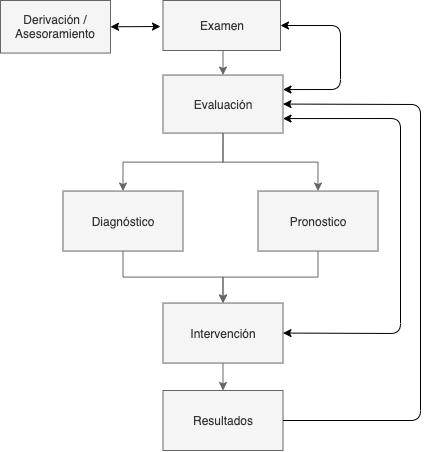
\includegraphics[scale=0.45]{imag/C4-Terapeuta.png}
\caption{Proceso de manejo de pacientes y usuarios por terapeuta. \textit{Guía para la práctica fisioterapéutica \cite{5}.}}
\label{2}
\end{figure}
\FloatBarrier

Es importante definir en que consisten los módulos representados para resolver principalmente el esquema de arquitectura que se definirá mas adelante.

\textbf{Examen}
\begin{itemize}
    \item La historia clínica: es una recopilación sistemática de datos, del pasado y del presente, relacionados con el motivo por el cual el paciente solicita los servicios de un fisioterapeuta
    \item Evaluación del sistema pulmonar: durante la fase de elaboración de la  historia clínica los fisioterapeutas solicitan información sobre el sistema pulmonar para determinar si hay síntomas que sugieran la necesidad de otra evaluación médica.
    \item Pruebas y parámetros: son los medios para recopilar datos sobre la persona y es la fase donde el fisioterapeuta decide los parámetros específicos que el paciente debe tener en cuenta para realizar una prueba de sistema pulmonar, con esta fase completada se puede emitir un diagnostico y pronóstico y determinar un plan de atención.
\end{itemize}

\textbf{Evaluación}
\begin{itemize}
    \item Interpretan la respuesta de la persona o paciente a las pruebas y parámetros
    \item Integran los datos de las pruebas y los parámetros con otra información recopilada al hacer la historia clínica
    \item Determinar un diagnóstico que pueda abordarse con el manejo por parte del fisioterapueta
    \item Determinar un pronóstico, que incluya objetivos para el manejo por parte del fisioterapeuta
    \item Elaborar un plan de atención
\end{itemize}

\textbf{Diagnóstico}
\newline
Recopilar y clasificar datos en categorías según el esquema de clasificación relevante para el profesional
\begin{itemize}
    \item Los esquemas de clasificación deben respetar los limites impuestos a la profesión por la ley que puede regular tipos de categorías de diagnóstico
    \item Las pruebas y los parámetros necesarios para confirmar el diagnóstico deben encontrarse dentro del ámbito legal 
\end{itemize}






\subsubsection{Sesión de Fisioterapia}

Una sesión de fisioterapia incluye los ejercicios, resultados, intervención y realimentación necesaria que un terapia de rehabilitación pulmonar de un paciente necesita. A continuación en la gráfica se presenta un modelo estándar de  volúmenes y capacidades pulmonares a partir de una traza de espirómetro. Las flechas negras y grises sólidas indican los volúmenes y capacidades pulmonares respectivamente. 


%explicar comportamiento de gráfico.



%Las técnicas de re-expansión pulmonar son utilizadas por los fisioterapeutas para mejorar los volúmenes y capacidades pulmonares de los pacientes. Para entender las técnicas es importante conocer los volúmenes y capacidades pulmonares, a continuación se presenta la descripción de los valores normales de volúmenes y capacidades pulmonares

%\begin{itemize}
 %   \item Volumen de reserva inspiratoria (VIR) : volumen que se puede respirar después de una inspiración normal, 3000 ml.
  %  \item Volumen corriente (TV): volumen inspirado y espirado con cada respiración, 500 ml.
   % \item Volumen de reserva espiratoria (ERV): volumen que puede expirar después de una respiración normal, 1100ml.
    %\item Volumen residual (RV) : volumen que queda en el pulmón después de la espiración máxima (no se puede medir mediante espirometría), 1200ml.
    %\item Capacidad inspiratoria (IC) : volumen que se puede respirar después de una exhalación normal, 3500 ml.
    %\item Capacidad residual funcional (CRF) : volumen que queda en los pulmones después de la espiración normal, 2300 ml.
    %\item Capacidad vital (VC) : volumen máximo que puede expirar después de la inspiración máxima, 4600 ml. 
    %\item Capacidad pulmonar total (TLC) : volumen de aire en los pulmones después de la inspiración máxima, 6000 ml.
    
%\end{itemize}

\begin{figure}[ht]
\centering
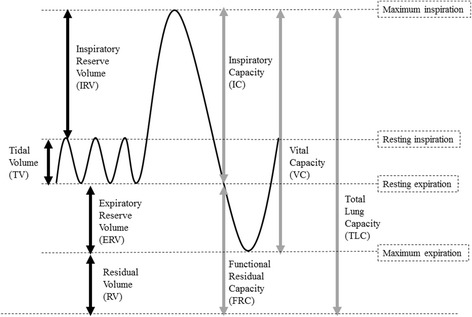
\includegraphics[scale=0.6]{imag/volumeslung.jpeg}
\caption{Medidas estándar de volumen pulmonar \cite{18}. }
\label{3}
\end{figure}
\FloatBarrier

%explicar proyecto


Este proyecto abarca con la posibilidad de que un fisioterapeuta pueda realizar una prescripción y luego pueda revisar los resultados de un incentivo respiratorio.

\subsubsection{Ejercicio de Fisioterapia para Paciente}

%complementar informacion

%A continuación se describen los tipos de ejercicios con sus características:

%\textbf{Patrón Diafragmático} \\
%Es un ejercicio que se encarga de lograr una capacidad residual funcional del paciente por medio de la inspiración nasal y espiración bucal. 


%\textbf{Inspiración Profunda}\\
%Es un ejercicio que se encarga de alcanzar la capacidad inspiratoria máxima (Volumen corriente VC + volumen de reserva inspiratorio VRI) mediante lo siguiente:
%\begin{itemize}
 %   \item Realizar una inspiración nasal lenta. 
  %  \item Realizar una apnea de 3 a 10 segundos. 
  %  \item Realizar una espiración lenta por la boca. 
%\end{itemize}

%\textbf{Inspiración fraccionada en el tiempo}\\
%La utilización de varias inspiraciones dentro del mismo ciclo ventilatorio, favorece la utilización de la capacidad inspiratoria en su plenitud con finalidad re-expansiva. Consiste en inspiraciones suaves y cortas por vía nasal e interrumpidas por cortos periodos de apnea (mínimo dos segundos cada uno) post inspiratoria programadas hasta en seis tiempos consecutivos, la espiración se da por la boca hasta el nivel de reposo inspiratorio o se extiende hasta el volumen medio de reserva inspiratoria.(4)
%El terapeuta determina en cuantas inspiraciones se llevará a cabo ya que puede ser inspiración fraccionada en 2 tiempo (realizar dos inspiraciones con los parámetros anteriores), en 3 tiempo 
%\begin{itemize}
 %   \item Inspiración nasal suave y corta
 %   \item Post inspiración realizar un periodo de apnea de mínimo dos segundos
 %   \item Se realizan hasta seis inspiraciones.
 %   \item Realizar una espiración suave por la boca
%\end{itemize}

%\textbf{Suspiros Inspiratorios}\\
%Este ejercicio se trata de una inspiración subdividida en inspiraciones cortas y sucesivas, sin apneas hasta que el paciente pueda contemplar la máxima capacidad inspiratoria




%\textbf{Espiración abreviada}\\
%Este ejercicio esta dado por 3 fases:
%\begin{itemize}
 %   \item Fase 1: Inspiración suave y profunda, espirando una pequeña cantidad de aire
  %  \item Fase 2: Vuelve a inspirar profundamente a partir del termino de la primera fase, espira nuevamente una pequeña cantidad de aire.
  %  \item Fase 3: vuelve a inspirar profundamente a partir del termino de la segunda fase, espirando completamente
%\end{itemize}



%\textbf{Ciclo Activo}\\
%Se encarga especialmente de repetir un ejercicio de patrón diafragmático o cualquiera de los ejercicios anteriores según el fisioterapeuta lo determine para el paciente asignado.











\subsubsection{Evaluación de Fisioterapia}

La evaluación de fisioterapia tiene en cuenta lo siguiente:

\begin{itemize}
    \item \textbf{Signos:} es algo que presenta el paciente y puede ser visto por terceros de forma objetiva.
    \item \textbf{Síntomas:} solamente son descritos por el paciente y no son observables. 
    \item \textbf{Auscultación:} Escuchar los ruidos del cuerpo de forma directa o con instrumentos como es estetoscopio.
    \item \textbf{Rayos x:} un examen médico no invasivo que ayuda a los médicos a diagnosticar y tratar las condiciones médicas. 
\end{itemize}


\subsubsection{Prescripción}

El fisioterapeuta puede realizar una prescripción con la asignación de las variables y  valores correspondientes


\textbf{Tratamiento de datos en una prescripción}

\begin{itemize}
    \item \textbf{Frecuencia:} Cada cuantas horas se debe realizar un ejercicio, es determinada por el fisioterapeuta y se define por el numero veces que realiza una sesión de fisioterapia, ejemplo: 3 series de 10 repeticiones, cada 8 horas, por una semana.
    \item \textbf{Duración:} Es el tiempo utilizado en la ejecución de una terapia.
    \item \textbf{Sesión:} Es la ejecución de un ejercicio en tiempo continuo en grupos de frecuencia.
    \item \textbf{Series:} Determinado por los momentos en una sola frecuencia.
    \item \textbf{Repeticiones:} Son las veces por serie de cada sesión
\end{itemize}
    
Un ejemplo de una prescripción es cuando un paciente necesita alcanzar el 50-70\% de Capacidad Vital (CV), en 3 series de 10 repeticiones con 1 minuto de descanso.


\begin{figure}[ht]
\centering
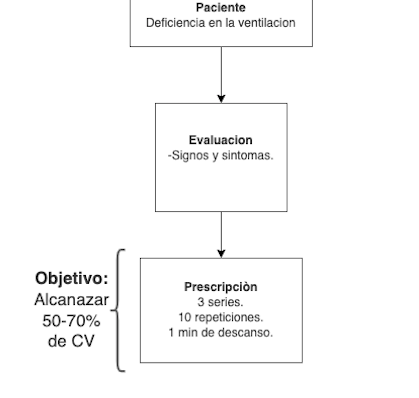
\includegraphics[scale=0.45]{imag/prescripcion.png}
\caption{Diagrama de contexto de sistema software de capacidad pulmonar. }
\label{4}
\end{figure}
\FloatBarrier






\subsubsection{Visualización de Datos de Espirometría}  %investigar

Los datos espirométricos se ven como gráficos llamados \textit{espirogramas} donde se muestran las medidas del volumen exhalado
en litros, el tiempo en segundos y las tasas de flujo de aire en litros por segundo. Hay dos tipos de espirogramas que se utilizan en la muestra de flujo respiratorio:

La visualización de datos de una sesión de Fisioterapia esta dada por: 

\begin{itemize}
    \item \textbf{Curva de Volumen-Tiempo}: Contiene los puntos de medición correspondientes a FEV1 y FEV.
        \begin{figure}[ht]
        \centering
        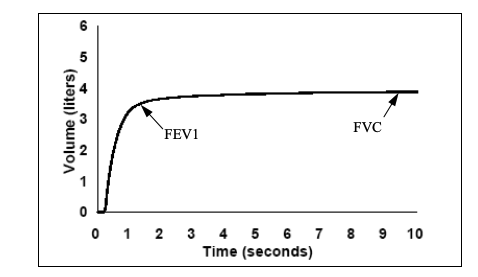
\includegraphics[scale=0.45]{imag/volumentiempo.png}
        \caption{Curva de Volumen / tiempo. }
        \label{4}
        \end{figure}
        \FloatBarrier

    
    \item \textbf{Curva de Flujo-Volumen}: Muestra las tasas de flujo de aire en función del volumen exhalado. Esta curva también contiene puntos correspondientes al PEF y FVC.
    
        \begin{figure}[ht]
        \centering
        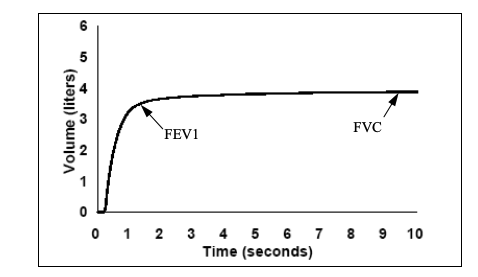
\includegraphics[scale=0.45]{imag/volumentiempo.png}
        \caption{Curva de Flujo / volumen. }
        \label{4}
        \end{figure}
        \FloatBarrier
    
    
\end{itemize}


Para la visualización de los datos en el proyecto se definió un rango de variación de flujo respiratorio de: [ 0 - 1200 ] centímetros cúbicos por segundo cc/s. Para el fisioterapeuta respiratorio, es importante conocer cuando el paciente ha logrado alcanzar 600, 900 y 1200 (cc/s).


\subsubsection{Resultados de una Terapia Respiratoria}

%Cada paciente o participante de una terapia respiratoria debe tener realimentación de los resultados media





%-------------------------------------------------------------------------------------

%capitulo aparte



\section{Metodología de la investigación}

La metodología considerada para el desarrollo del proyecto es TRIZ lo cual nos permite clasificar los atributos y características para definir los requerimientos del sistema inspirómetro, esta metodología se desarrolla en conjunto con el grupo de investigación de la Pontificia Universidad Javeriana Cali donde se integran áreas de fisioterapia, ingeniería de sistemas, ingeniería electrónica, diseño, ingeniería de software para desarrollar un sistema que permita realizar una terapia respiratoria y tenga realimentación visual para los usuarios, se plantea entonces los atributos del sistema en pasado, presente y futuro en nueve ventanas.

\begin{figure}[ht]
\centering
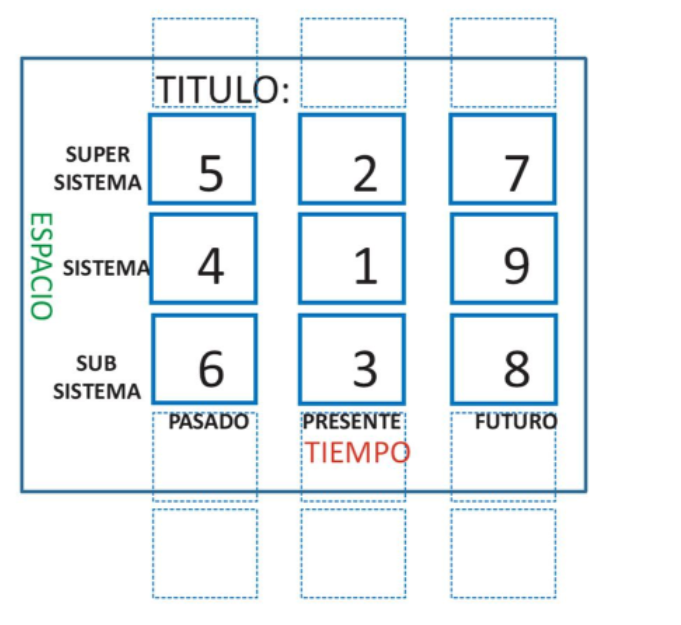
\includegraphics[scale=0.45]{imag/9ventanas.png}
\caption{Diagrama de nueve ventanas de metodología TRIZ }
\label{4}
\end{figure}
\FloatBarrier


%fases de la metodología en diagrama %deio

%\subsection{Sistema presente} 

%\subsubsection{Ventana 1}
%En esta ventana se analizaron los diferentes elementos de ayuda para la recuperación pulmonar de un paciente con sistemas actuales, se identifica que estos sistemas siempre van acompañados de una terapia denominada fisioterapia respiratoria, que como se explico anteriormente, es la encargada de definir que tipo de terapia es la mejor para cada complicación respiratoria.

%que se obtuvo en cada una de las fases, el proyecto grande utilizo las nueve ventanas despues de ello surgio la arquitectura de referencia, seccion global, proyecto grande, contar resultados resumidos, requesitos genericos y luego el desarrollo de software, 

%\subsubsection{Ventana 2} 

%Se realiza el  análisis del supersistema, lo cual es en contexto donde se describen los elementos de ayuda para la recuperación de la capacidad pulmonar, en esta ventana se analizan las entidades o empresas que trabajan en la recuperación de la salud respiratoria, como también otros sectores relacionados con complicaciones respiratorias. 

%En medicina, se utiliza respiración asistida en procesamientos quirúrgicos, donde se tienen en cuenta también técnicas respiratorias y fármacos para personas con enfermedades pulmonares. En industria, existen empresas que realizan el diseño y construcción de áreas limpias, manejo y control de ambientes hospitalarios y farmacéuticos. En lo social, esta directamente relacionado con el contagio de COVID por las personas que necesitan un tratamiento respiratorio asistido.

%\subsubsection{Ventana 3}

%Se realiza el  análisis del subsistema, donde se muestra de que están compuestos los diferentes elementos  investigados asociados a la recuperación de la capacidad pulmonar. Actualmente, se utilizan técnicas para la recuperación pulmonar de las personas, que se basan en una serie de instrucciones que el paciente debe seguir de acuerdo a la recomendación médica. Con un inspirómetro un paciente debe inhalar a través de la boquilla, lo que hace que la presión caiga dentro del dispositivo y, a su vez, hace que las bolas se eleven en cada uno de los tubos de flujo. Cada tubo está calibrado para que el desplazamiento completo de la pelota sea igual a un flujo específico, que se indica en la pared del tubo. El número de bolas y el nivel al que se elevan depende del nivel de flujo alcanzado. 

%https://patentimages.storage.googleapis.com/e3/b0/03/fefa9df55c113e/US20190134460A1.pdf

% investigar a nivel de software


%Durante el análisis de la metodologías utilizadas en sistemas actuales, se identifica que una terapia respiratoria no se realiza adecuadamente debido a la falta de adherencia hacia la actividad por parte del paciente, además no existe un seguimiento con datos registrados que el terapeuta pueda evaluar, no hay un registro tampoco de un histórico de la evolución del paciente quien requiere principalmente indicaciones previas del terapeuta respiratorio.

%\subsection{Sistema pasado}

%\subsubsection{Ventana 4}

%La rehabilitación pulmonar abarca desde los comienzos del arte médico, con ello, las principales estrategias utilizadas para disminuir el impacto de la enfermedad pulmonar crónica, las terapias recomendadas eran el reposo, evitar situaciones de esfuerzo físico o por el contrario entrenamientos físico con miras a rehabilitar los pacientes con el máximo posible de alcance de su sistema pulmonar y después de ello, también se desarrollaron técnicas aplicando los principios científicos entre los cuales vemos el entrenamiento muscular y oxígeno-terapia crónica domiciliaria.

%\subsubsection{Ventana 5}

%En el pasado no se tenía la conciencia de prevenir ciertos tipos de enfermedades como las respiratorias, de hecho no existían grandes compañías dedicadas al cuidado o rehabilitación de la capacidad pulmonar como las hay hoy en día. Solo existían esfuerzos e investigaciones individuales cuyas conclusiones permitieron que se desarrolle la industria que actualmente existe.

%\subsubsection{Ventana 6}

%Debido a que el pasado no existía una gran preocupación sobre enfermedades respiratorias y en general como las hay hoy en día, no había dispositivos que ayudaran a la recuperación pulmonar de las personas, salvo ejercicios de respiración que aún se usan en la fisioterapia respiratoria. 




%\subsection{Sistema futuro} 

%\subsubsection{Ventana 7}

%En cuanto al futuro se entra al plano imaginario, en este caso el contexto en el que se encontraran los elementos de recuperación pulmonar. 
%En medicina uno de los aspectos a mejorar es la de la reducción de tiempos de convalecencia en los hospitales porque minimiza costos tanto al hospital como al paciente además abre espacio para pacientes con otras patologías y una de las tendencias para lograr esto es la fisioterapia domiciliaria, que el paciente realice su terapia desde la comodidad de su casa y no tenga de desplazarse hasta el hospital. Desde lo social y ambiental, estos temas van de la mano debido a que en algunos países no se está trabajando lo suficiente en lo ambiental lo cual significa un aumento en la contaminación del aire que respiran las personas sobre todo en las grandes ciudades, lo cual también aumentaría la probabilidad de adquirir algunas afección respiratoria y sin tratamiento podría aumentar la tasa de mortalidad por estas causas. 

%\subsubsection{Ventana 8}

%El sistema ideado deberá usar algoritmos de programación para el envío y recepción de datos además de generar un reporte de datos de lo realizado por el paciente en el cual el profesional de la salud analizará el rendimiento del paciente.

%\subsubsection{Ventana 9}

%El software del inspirómetro deberá ser capaz de ejecutarse en el sistema operativo más usado en el mundo, con el fin de tener mayores posibilidades de uso.  Además deberá tener una interfaz gráfica intuitiva para que tanto el paciente como el terapeuta puedan usarlo de manera fácil y adecuada. Dicha interfaz deberá permitir modificar los límites de trabajo por parte del terapeuta con el fin de adaptar la terapia a los pacientes con mayores dificultades respiratorias. 


%Dadas las características y atributos de los sistemas en pasado y presente, el sistema futuro, debe permitir que el paciente se pueda concentrar en su terapia y hacerla conscientemente, permitir adquirir datos, codificar, presentar y almacenar la información de desempeño de la terapia tanto al paciente como al terapeuta mediante una conexión remota, debe permitir la administración de usuarios, una plataforma con operaciones intuitivas para la programación de ejercicios para cada sesión y que permita la prescripción remoto de los mismos.

%-------------------------------------------------------------------------------------
\section{Proceso de Ingeniería de Software  } %desarrollo del software (perfil del terapueta)

%incluir diagrama de casos de uso con explicación

Bajo los atributos identificados con la metodología TRIZ se desarrollan a continuación los requerimientos funcionales y no funcionales del sistema software propuesto.


\subsection{Definición de requisitos del sistema}

En esta sección se detallan los procesos realizados para obtener los requisitos del sistema, la estructura y documentación de los requisitos, validación y priorización de estos.

\subsubsection{Diagrama de contexto} %explicar 

Contiene todos los posibles escenarios, personas, documentación que interactúan, aportan datos e información para el sistema software del inspirómetro también se identifican zonas grises sobre una posible regulación de tratamiento de datos que fueron definidos por las partes interesadas para la construcción de la aplicación.

\begin{figure}[ht]
\centering
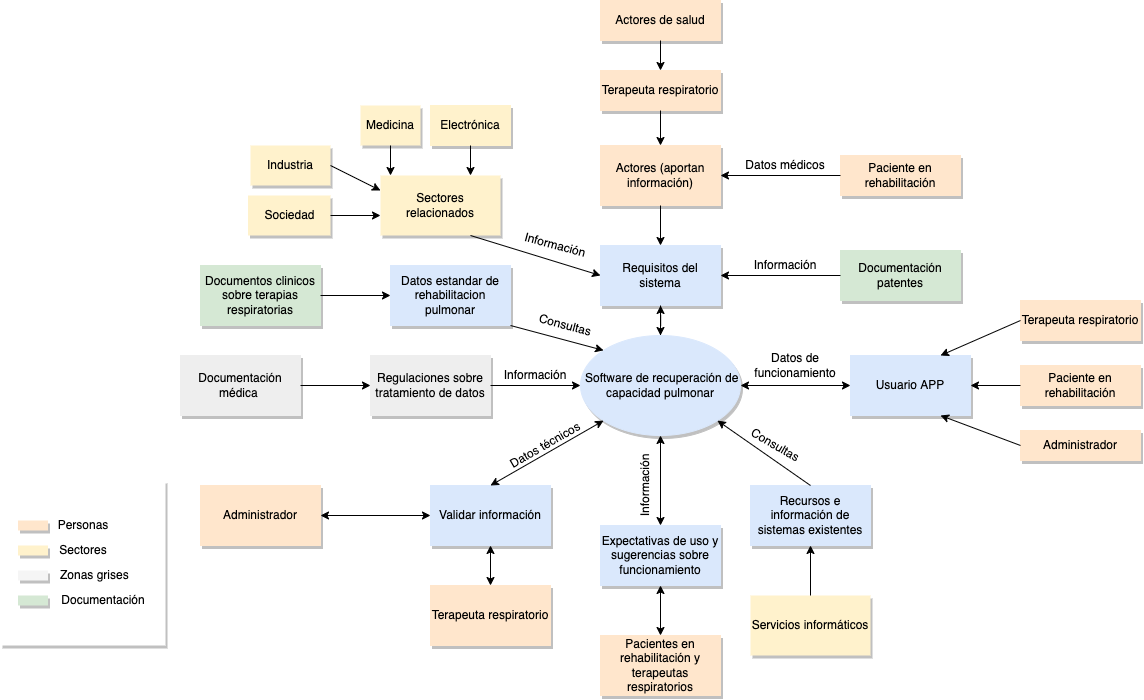
\includegraphics[scale=0.40]{imag/C4-Diagram contexto.drawio.png}
\caption{Diagrama de contexto de sistema software de inspirómetro. }
\label{4}
\end{figure}
\FloatBarrier

\newpage

\subsubsection{Diagrama de Casos de Uso} %explicar 

Se identificaron las posibles relaciones mediante un diagrama de casos de usos que permitió exponer el comportamiento deseado del sistema. En la siguiente figura se muestra la inclusión de los procesos que incorpora explícitamente el comportamiento de un caso de uso, como también se muestra la extensión como sub-funciones de un caso de usos.


\begin{figure}[ht]
\centering
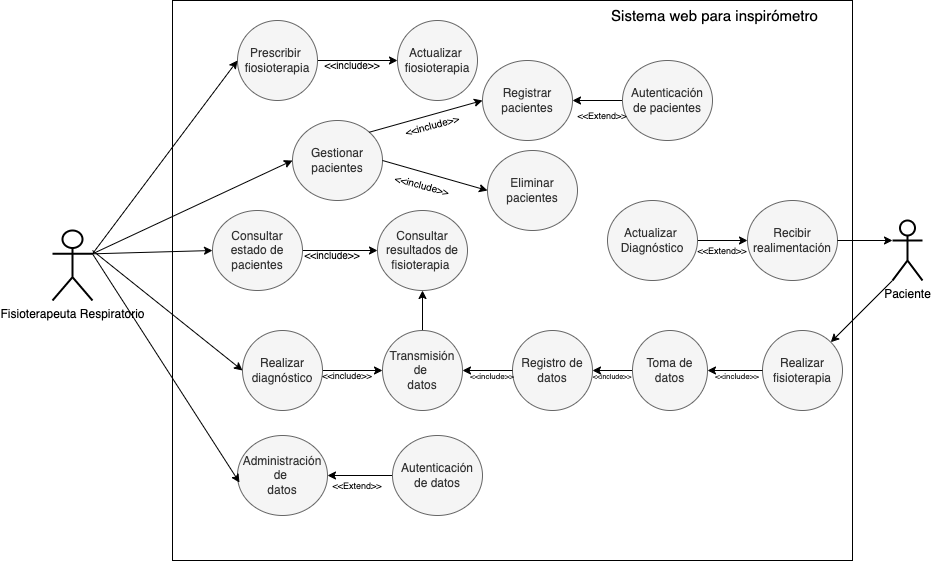
\includegraphics[scale=0.45]{imag/casosdeusof.png}
\caption{Diagrama de casos de uso para aplicación web }
\label{5}
\end{figure}
\FloatBarrier


\subsubsection{Diagrama de Flujo General del Aplicación Web} %explicar 

Como parte de las tareas principales que debe realizar el fisioterapeuta es la de asignar una prescripción y valorar el paciente dada la gráfica de comportamiento del flujo respiratorio que envía el inspirómetro a la aplicación web. Se presenta a continuación el diagrama de flujo cuando el fisioterapeuta ingresa a la aplicación web. 


\begin{figure}[ht]
\centering
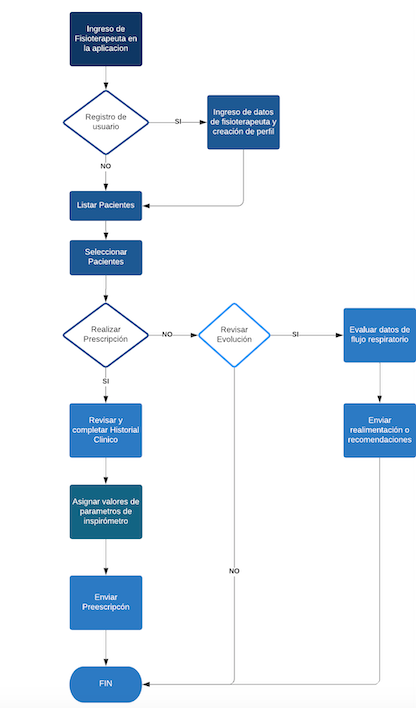
\includegraphics[scale=0.45]{imag/DiagramaFlujo.png}
\caption{Diagrama de flujo general para sistema web }
\label{5}
\end{figure}
\FloatBarrier


\newpage

\subsubsection{Técnicas de obtención de requisitos}

\begin{enumerate}
    \item \textbf{Reuniones grupales:} Inicialmente ser realizan reuniones grupales con los principales actores del sistema, tanto los posibles usuarios como terapeuta respiratorio como los desarrolladores del sistema de las diferentes áreas, software, electrónica y diseño
    \item \textbf{Encuestas:} 
        \begin{enumerate}
            \item Encuesta dirigida a fisioterapeutas tanto externos como internos del proyecto, con el propósito de identificar atributos comunes con los mencionados en el grupo de investigación, para lograr el objetivo, se realizaron preguntas orientadas a las terapias respiratorias, los datos que se evalúan actualmente y las metodologías utilizadas.
            \item Encuesta dirigida a los pacientes con el fin de conocer la experiencia de los pacientes que han realizado terapia respiratoria con el inspirómetro incentivo en cuanto a la terapia y el acompañamiento con el terapeuta.
        \end{enumerate}
        
    \item \textbf{Prototipado:} 
    
        \begin{enumerate}
            \item Se definieron vistas e interacción de usuario, en este caso, como el fisioterapeuta deberá desenvolver en la aplicación web, como el registro de pacientes, realización de la prescripción y la visualización de resultados para el diagnostico.
        \end{enumerate}
    
    
\end{enumerate}




\subsubsection{Definición de requisitos funcionales}

%Modulo Fisioterapeuta============================================ 

 % FUNCIÓN EVALUAR
\begin{enumerate}[start=1,label={\bfseries RF0\arabic*.}]

    \item El sistema debe tener una funcionalidad para el fisioterapeuta respiratorio que le permita evaluar el estado de un paciente. 
    %para una sesión realizada por un paciente 
        \label{RF01}
            \begin{enumerate}[label*=\arabic*.]
                %datos específicos evalúa el fisio
                \item Permitir realizar un diagnostico y posteriormente recetar la terapia correspondiente por paciente, si es necesario.
                
                \item Permitir la visualización de datos registrados como flujo respiratorio por cada sesión por medio de gráficas de desempeño.
                
                \item Permitir revisar la evolución del paciente dados los datos de flujo respiratorio de cada una de las terapias por sesión.
        
            \end{enumerate}

    %EJERCICIOS     --como quedan descritos? animaciones, textos ?
    \item El sistema debe tener una funcionalidad para al fisioterapeuta que le permita programar  una prescripción por cada sesión en el sistema web.
        
        \label{RF02}
            \begin{enumerate}[label*=\arabic*.]
            
                \item Se debe permitir cargar una prescripción con valores numéricos enteros. %completar si son descritos, texto o con animaciones
                 
                \item Se debe permitir el almacenamiento de prescripciones con valores asignados por paciente. %completar
                
                \item Se debe permitir modificar, cargar o eliminar prescripciones.
                
                \item Se debe permitir establecer parámetros de prescripciones por conexión remota.
                
     
                
            \end{enumerate}
            
    %ORIENTAR
    \item  El sistema debe tener una funcionalidad para al fisioterapeuta que le permita orientarse en el manejo de las prescripciones.
    
    \label{RF03}
            \begin{enumerate}[label*=\arabic*.]
                %Posible requerimiento
                \item Se debe incluir una función de usuario que permita ver una secuencia de uso de la aplicación correctamente. 
            \end{enumerate}
            
    
    %PACIENTES
    \item  El sistema debe tener una funcionalidad para al fisioterapeuta que le permita la gestión de los parámetros de cada sesión por medio de los perfiles de cada paciente, parámetros tales como  el rango de medición de flujo inspirado, volumen, frecuencia respiratoria y saturación de oxigeno por cada paciente. %preguntar       
    \label{RF04}
            \begin{enumerate}[label*=\arabic*.]
                \item La funcionalidad de gestión de parámetros que le permita al fisioterapeuta establecer rangos en volumen, frecuencia y saturación de oxigeno por medio de teleconsulta. %videollamada?
                
                \item La funcionalidad para al fisioterapeuta debe permitir establecer parámetros de flujo inspirado y asignar los ejercicios correspondientes por paciente
                
                
            \end{enumerate}
            
    %DIAGNOSTICO
    \item El sistema debe tener una funcionalidad para al fisioterapeuta que le permita realizar un diagnostico dados los datos de flujo respiratorio del paciente visualizados en gráficas de comportamiento.
    
    \item  El sistema debe tener una funcionalidad de envió de vídeos para brindar realimentaciones de manera cualitativa e instrucciones necesarias para la terapia.
    
    
    %ALMACENAR DATOS
    \item El sistema debe tener una funcionalidad para al fisioterapeuta que le permita guardar los cambios realizados en la plataforma como las modificaciones de las prescripciones en cada una de las sesiones de terapia.
    
    
    
            
%Modulo Paciente===================================================================

 %ORIENTAR
    \item El sistema debe tener una funcionalidad que permita orientar al paciente  para la realización de un ejercicio de una terapia respiratoria. 
    \label{RF08}
            \begin{enumerate}[label*=\arabic*.]
            
                \item La funcionalidad de orientar al paciente debe incluir una demostración con los pasos o secuencia a seguir sobre como manejar la aplicación, como usar el inspirómetro electrónico y como realizar el ejercicio prescrito.
                
                \item La funcionalidad de orientar al paciente de manera sensitiva debe permitir generar una secuencia en la terapia por cada sesión establecida al paciente, los ejercicios permitirán el estimulo que el paciente  necesita para su recuperación. %que serían las cualidades de la orientación
                
                \item La funcionalidad de orientar al paciente debe contar con una guía de usuario que debe incluir una demostración con los pasos o secuencia a seguir sobre como manejar la aplicación.
                
                \item La funcionalidad de orientar al paciente debe contar con un realimentación después de una sesión realizada que permita dar a conocer resultados y consejos de avance en terapia para una próxima sesión, esta funcionalidad se dará con la intervención del terapeuta al finalizar cada sesión.
    
                \item La funcionalidad de orientar al paciente debe mostrar datos de evolución que permitan conocer el estado en que se encuentra el paciente para completar una terapia respiratoria.
                
                \item La funcionalidad de orientar al paciente debe contar con una guía sobre como usar el inspirómetro electrónico y como realizar el ejercicio prescrito, resaltando también los limites de seguridad del sistema.
            \end{enumerate}
            
            
        %enviar realimentacion por otros medios no solo visual

%Modulo de  Administración============================================    

 
    \item El sistema debe contar con una estructura de gestión de usuarios.
    %Grupos de pacientes  
    \item El sistema debe permitir a los fisioterapeutas administrar grupos de pacientes para asignar las respectivas prescripciones.
    \label{RF10}
        \begin{enumerate}[label*=\arabic*.]
            \item Permitir a los fisioterapeutas la creación y administración de grupos de pacientes, los cuales van a tener en su plataforma registrados con los datos demográficos de cada paciente.
            
        \end{enumerate}
        
  
            

         
    
%Modulo sistema central de procesamiento===========================================
 
    
    %Adquirir datos
    
    \item El sistema debe permitir adquirir, almacenar y presentar al fisioterapeuta los datos de flujo respiratorio  como desempeño del paciente estimados en una sesión por conexión remota.
    
     \label{RF12}
            \begin{enumerate}[label*=\arabic*.]
                
                \item El sistema debe tener una funcionalidad de toma de datos de flujo respiratorio del paciente que permita agrupar la captura de datos en un historial.
                
                \item El sistema debe tener una funcionalidad de toma de datos del paciente que permita hacer el registro de datos de flujo respiratorio mediante los estímulos capturados uno a uno desde el inspirómetro con un método cuantitativo de grabación de datos.  %evaluar
                
                \item El sistema debe tener una funcionalidad de codificar la variable física medida con el inspirómetro a partir de los datos derivados del flujo respiratorio y presentarlos graficados en la aplicación web. %Codificar la información de la variable física medida. (estructura de datos)
            
            \end{enumerate}
        

      
    %Trasmisión de datos=================================
    
    
    \item El sistema debe contar con una API para permitir la trasmisión de datos.
    
   
    
    %Almacenamiento de datos
    
   
    \item El sistema debe permitir la funcionalidad de toma de datos del paciente debe garantizar el auto-guardado por cada actividad realizada.
    
    
  
    
    
    %Gamificación
    \item El sistema web debe permitir integrar un modulo de gamificación para acoplarse con un sistema móvil para la presentación de  prescripciones y  de datos de comportamiento de  flujo respiratorio.
    
     
    
    %%Juego
    \item El sistema debe permitir mantener un flujo  respiratorio constante indicado en los ejercicios prescritos por el fisioterapeuta.
    %porque eso le va a permitir que el flujo de aire llegue a los alveolos y realice el íntercambio, La parte de ser constante y laminar hace que la bolita o lo que se mira en el incentivo, Este quieta en un solo lugar, Sin subir o bajar,Entonces esa bolita quieta y a la altura  me permite saber que si lo esta haciendo bien, Si, pues dependiendo del volumen a donde el profesional le indique a la persona llegar. Ya que el dispositivo tiene aun lado marcado como en rayitas los niveles de volumen que se esta alcanzando
    \label{RF21}
            \begin{enumerate}[label*=\arabic*.]
            
                \item El sistema debe permitir la funcionalidad de mantener un flujo y volumen constante en cada sesión para registrar los niveles de volumen y frecuencia respiratoria 
            \end{enumerate}
    
        

%https://www.gloomaps.com/3zr2f3aYfo

\end{enumerate}


\subsubsection{Definición de requisitos no funcionales}

\begin{enumerate}[start=1,label={\bfseries RNF\arabic*.}]


\item  El sistema no debe ser exigente en tecnología para que pueda ser usado por cualquier paciente con un sistema tecnológico de comunicación. %Android

\item El sistema debe estar en la capacidad de funcionar en modo offline, es decir soporte sin conexión, cuando las condiciones de conexión con el servidor sean adversas, asegurando que la información no se pierda a causa de estos imprevistos

\item El sistema debe permitir que cualquier usuario que no conozca a profundidad el funcionamiento de las TIC tenga un buen desempeño con el manejo de la herramienta

\item El sistema debe asegurar una disponibilidad del 99.0 \%

\item El sistema debe ser desarrollado bajo los principios de diseño SOLID

\item El sistema debe tener un tiempo TTI menor o igual a 5 segundos

 \item El sistema debe cumplir con parámetros ACID para el relacionamiento con bases de datos
 
\item El sistema debe contar con las características necesarias para hacer un deploy sencillo

\item El sistema debe contar con una función de backup y de recuperación ante fallos
\item El sistema debe soportar concurrencia de múltiples usuarios
\item El sistema debe contar con los protocolos necesarios para asegurar un funcionamiento seguro a través de Internet, es decir, que la información enviada y recibida este protegida contra ataques de robo información y suplantación de identidad. 
\item El sistema no debería ser invasivo.
        
\item El sistema debe favorecer la adherencia al tratamiento de fisioterapia.

\end{enumerate}




\subsubsection{Definición de requisitos tipo restricción}

\begin{enumerate}[start=1,label={\bfseries RTR\arabic*.}]

\item Poner el mínimo número de comandos de operación para el paciente.


\end{enumerate}


\subsubsection{Priorización de Requisitos}
%-------------------------------------------------------------------------------------

A continuación se presenta los requisitos funcionales con su respectiva especificación y validación dependiendo del la prioridad: alta, media o baja, respectivamente.


\begin{center}
\begin{tabular}{|c|c|p{4cm}|p{4cm}|}
            \hline
            \rowcolor{red} \multicolumn{4}{|c|}{\textbf{Prioridad:} Alta}  \\
            \hline
            \multicolumn{2}{|l}{\textbf{Nro.Requisito: }RF.01} & \multicolumn{1}{|l}{\textbf{Versión: 1.1}} & \multicolumn{1}{|l|}{\textbf{Estado: Aprobado}} \\
            \multicolumn{4}{|p{13cm}|}{\textbf{Caso de uso Nro: }}  \\
            \hline
            \multicolumn{4}{|p{13cm}|}{\textbf{Descripción: } El sistema debe tener una funcionalidad para el terapeuta respiratorio que le permita evaluar una sesión realizada por un paciente } \\
            \multicolumn{4}{|p{13cm}|}{\textbf{Justificación: } El fisioterapeuta solicita que la aplicación web le permita ver los datos del paciente y conocer la evolución del mismo.} \\ 
            \multicolumn{4}{|p{13cm}|}{\textbf{Origen: }Fisioterapeuta}  \\
            \multicolumn{4}{|p{13cm}|}{\textbf{Criterio de verificación: } El sistema web permite visualizar los datos registrados de una prescripción y conocer la evolución del paciente.  } \\
            \hline
            \multicolumn{4}{|p{13cm}|}{\textbf{Prerequisitos: } Todos los requisitos de prioridad alta. }\\
            \hline \multicolumn{4}{|p{12cm}|}{\textbf{Dependencias: }
                \begin{itemize}
                \item RF01.1
                \item RF01.2
                \item RF01.3
                \end{itemize}}  \\
            \multicolumn{4}{|p{12cm}|}{\textbf{Conflictos: }}  \\
            \hline
            \multicolumn{4}{|p{12cm}|}{\textbf{Documentos de soporte: }}  \\
            \hline
            \multicolumn{4}{|p{12cm}|}{\textbf{Historial del Requerimiento: }}  \\
            \multicolumn{4}{|p{12cm}|}{\textbf{Creación : }09/10/2021}  \\
            \multicolumn{4}{|p{12cm}|}{\textbf{Modificación: }}  \\
             \textbf{Versión} & \textbf{Fecha} & \multicolumn{2}{p{8cm}|}{\textbf{Cambio realizado:}} \\
            \hline
               1.1    &20/10/2021 &   \multicolumn{2}{p{8cm}|}{Se desarrolla prototipado para esta funcionalidad y se modifica los requisitos RF01.2 y RF01.3 en cuanto a visualizar los datos como flujo respiratorio y se crea el requisito RF01.1}
              \\
            \hline
        \end{tabular}

        
        \medskip
        
        
        %%%%%%%%%%%%%%%%%%%%%%%%%%%%%%%%%%%%%2
        
        
        \begin{tabular}{|c|c|p{4cm}|p{4cm}|}
            \hline
            \rowcolor{red} \multicolumn{4}{|c|}{\textbf{Prioridad:} Alta}  \\
            \hline
            \multicolumn{2}{|l}{\textbf{Nro.Requisito: }RF.02} & \multicolumn{1}{|l}{\textbf{Versión: 1.1}} & \multicolumn{1}{|l|}{\textbf{Estado: Aprobado}} \\
            \multicolumn{4}{|p{13cm}|}{\textbf{Caso de uso Nro: }}  \\
            \hline
            \multicolumn{4}{|p{13cm}|}{\textbf{Descripción: } El sistema debe tener una funcionalidad para el terapeuta respiratorio que le permita programar una prescripción por cada sesión en el sistema web } \\
            \multicolumn{4}{|p{13cm}|}{\textbf{Justificación: } El fisioterapeuta solicita que la aplicación web le permita programar una prescripción general por paciente.} \\ 
            \multicolumn{4}{|p{13cm}|}{\textbf{Origen: }Fisioterapeuta}  \\
            \multicolumn{4}{|p{13cm}|}{\textbf{Criterio de verificación: } El sistema web permite visualizar los datos registrados de una prescripción y conocer la evolución del paciente.  } \\
            \hline
            \multicolumn{4}{|p{13cm}|}{\textbf{Prerequisitos: } Todos los requisitos de prioridad alta. }\\
            \hline \multicolumn{4}{|p{12cm}|}{\textbf{Dependencias: }
                \begin{itemize}
                \item RF02.1
                \item RF02.2
                \item RF02.3
                \item RF02.4
                \end{itemize}}  \\
            \multicolumn{4}{|p{12cm}|}{\textbf{Conflictos: }}  \\
            \hline
            \multicolumn{4}{|p{12cm}|}{\textbf{Documentos de soporte: }}  \\
            \hline
            \multicolumn{4}{|p{12cm}|}{\textbf{Historial del Requerimiento: }}  \\
            \multicolumn{4}{|p{12cm}|}{\textbf{Creación : }09/10/2021}  \\
            \multicolumn{4}{|p{12cm}|}{\textbf{Modificación: }}  \\
             \textbf{Versión} & \textbf{Fecha} & \multicolumn{2}{p{8cm}|}{\textbf{Cambio realizado:}} \\
            \hline
               1.1    &20/10/2021 &   \multicolumn{2}{p{8cm}|}{Se desarrolla prototipado para esta funcionalidad y se modifica los requisitos RF02.1 y RF02.2 en cuanto a realizar una prescripción con campos para valores numéricos}
              \\
            \hline
        \end{tabular}

        
   %     \medskip
        
        
        
        
        
        
        %%%%%%%%%%%%%%%%%%%%%%%%%%%%%%%%%%%%
        
         \begin{tabular}{|c|c|p{4cm}|p{4cm}|}
            \hline
            \rowcolor{orange} \multicolumn{4}{|c|}{\textbf{Prioridad:} Media}  \\
            \hline
            \multicolumn{2}{|l}{\textbf{Nro.Requisito: }RF.03} & \multicolumn{1}{l|}{\textbf{Versión: }} & \multicolumn{1}{|l|}{\textbf{Estado: Aprobado}} \\
            \multicolumn{4}{|p{12cm}|}{\textbf{Caso de uso Nro: }}  \\
            \hline
            \multicolumn{4}{|p{13cm}|}{\textbf{Descripción: } El sistema debe tener una funcionalidad para al fisioterapeuta que le permita orientarse en el manejo de las prescripciones}  \\
            \multicolumn{4}{|p{13cm}|}{\textbf{Justificación: }Se sugiere al fisioterapeuta conocer la secuencia de pantallas de la interfaz web y como se esperan los datos}  \\
            \multicolumn{4}{|p{12cm}|}{\textbf{Origen: }Ingeniero de requisitos}  \\
            \multicolumn{4}{|p{13cm}|}{\textbf{Criterio de verificación: }}  \\
            \hline
            \multicolumn{4}{|p{13cm}|}{\textbf{Prerequisitos: }}  \\
            \hline
            \multicolumn{4}{|p{12cm}|}{\textbf{Dependencias: }
                \begin{itemize}
                \item RF03.1
                \end{itemize}}  \\
            \multicolumn{4}{|p{12cm}|}{\textbf{Conflictos: }}  \\
            \hline
            \multicolumn{4}{|p{12cm}|}{\textbf{Documentos de soporte: }}  \\
            \hline
            \multicolumn{4}{|p{12cm}|}{\textbf{Historial del Requerimiento: }}  \\
            \multicolumn{4}{|p{12cm}|}{\textbf{Creación : }20/09/2021}  \\
            \multicolumn{4}{|p{12cm}|}{\textbf{Modificación: }}  \\
             \textbf{Versión} & \textbf{Fecha} & \multicolumn{2}{p{8cm}|}{\textbf{Cambio realizado:}} \\
            \hline
               1.1    &31/10/2021 &   \multicolumn{2}{p{8cm}|}{se desarrolla prototipado para esta funcionalidad y se modifica el requisito RF03.1 en cuanto a orientar al fisioterapeuta}
              \\
            \hline
        \end{tabular}
        
        
        \begin{tabular}{|c|c|p{4cm}|p{4cm}|}
            \hline
            \rowcolor{yellow} \multicolumn{4}{|c|}{\textbf{Prioridad:} Baja}  \\
            \hline
            \multicolumn{2}{|l}{\textbf{Nro.Requisito: }RF.04} & \multicolumn{1}{l|}{\textbf{Versión: 1.1 }} & \multicolumn{1}{|l|}{\textbf{Estado: Aprobado}}  \\
            \multicolumn{4}{|p{12cm}|}{\textbf{Caso de uso Nro: }}  \\
            \hline
            \multicolumn{4}{|p{13cm}|}{\textbf{Descripción: }El sistema debe tener una funcionalidad para al fisioterapeuta que le permita la gestión de los parámetros de cada sesión por medio de los perfiles de cada paciente, parámetros tales como el rango de medición de flujo inspirado, volumen, frecuencia respiratoria por cada paciente.}  \\
            \multicolumn{4}{|p{13cm}|}{\textbf{Justificación: }El Fisioterapeuta solicita que la aplicación web le permita la gestión de parámetros para realizar una prescripción}  \\
            \multicolumn{4}{|p{12cm}|}{\textbf{Origen: }Fisioterapeuta}  \\
            \multicolumn{4}{|p{13cm}|}{\textbf{Criterio de verificación: }}  \\
            \hline
            \multicolumn{4}{|p{13cm}|}{\textbf{Prerequisitos: }}  \\
            \hline \multicolumn{4}{|p{12cm}|}{\textbf{Dependencias: }
                \begin{itemize}
                \item RF04.1
                \item RF04.2
                \end{itemize}}  \\
            \multicolumn{4}{|p{12cm}|}{\textbf{Conflictos: }}  \\
            \hline
            \multicolumn{4}{|p{12cm}|}{\textbf{Documentos de soporte: }}  \\
            \hline
            \multicolumn{4}{|p{12cm}|}{\textbf{Historial del Requerimiento: }}  \\
            \multicolumn{4}{|p{12cm}|}{\textbf{Creación : }20/09/2021}  \\
            \multicolumn{4}{|p{12cm}|}{\textbf{Modificación: }}  \\
             \textbf{Versión} & \textbf{Fecha} & \multicolumn{2}{p{8cm}|}{\textbf{Cambio realizado:}} \\
            \hline
               1.1    &31/10/2021 &   \multicolumn{2}{p{8cm}|}{Se desarrolla prototipado para esta funcionalidad y se modifica los requisitos RF04.1 en cuanto a establecer parámetros generales de prescripción y se crea el requisito RF04.2}
              \\
            \hline
        \end{tabular}
        
        

\begin{tabular}{|c|c|p{4cm}|p{4cm}|}
            \hline
            \rowcolor{red} \multicolumn{4}{|c|}{\textbf{Prioridad:} Alta}  \\
            \hline
            \multicolumn{2}{|l}{\textbf{Nro.Requisito: }RF.05} & \multicolumn{1}{|l}{\textbf{Versión: 1.1}} & \multicolumn{1}{|l|}{\textbf{Estado: Aprobado}} \\
            \multicolumn{4}{|p{13cm}|}{\textbf{Caso de uso Nro: }}  \\
            \hline
            \multicolumn{4}{|p{13cm}|}{\textbf{Descripción: } El sistema debe tener una funcionalidad para al fisioterapeuta que le permita realizar un diagnostico dados los datos de flujo respiratorio del paciente visualizados en gráficas de comportamiento. } \\
            \multicolumn{4}{|p{13cm}|}{\textbf{Justificación: } El fisioterapeuta solicita que la aplicación web le permita ver el comportamiento de flujo respiratorio del paciente y conocer la evolución del mismo.} \\ 
            \multicolumn{4}{|p{13cm}|}{\textbf{Origen: }Fisioterapeuta}  \\
            \multicolumn{4}{|p{13cm}|}{\textbf{Criterio de verificación: } El sistema web permite visualizar los datos de flujo respiratorio del paciente.  } \\
            \hline
            \multicolumn{4}{|p{13cm}|}{\textbf{Prerequisitos: } Todos los requisitos de prioridad alta. }\\
            \hline \multicolumn{4}{|p{12cm}|}{\textbf{Dependencias: }
                }  \\
            \multicolumn{4}{|p{12cm}|}{\textbf{Conflictos: }}  \\
            \hline
            \multicolumn{4}{|p{12cm}|}{\textbf{Documentos de soporte: }}  \\
            \hline
            \multicolumn{4}{|p{12cm}|}{\textbf{Historial del Requerimiento: }}  \\
            \multicolumn{4}{|p{12cm}|}{\textbf{Creación : }09/10/2021}  \\
            \multicolumn{4}{|p{12cm}|}{\textbf{Modificación: }}  \\
             \textbf{Versión} & \textbf{Fecha} & \multicolumn{2}{p{8cm}|}{\textbf{Cambio realizado:}} \\
            \hline
               1.1    &20/10/2021 &   \multicolumn{2}{p{8cm}|}{Se desarrolla prototipado para esta funcionalidad y  se modifica los requisitos RF05 en cuanto a visualizar los datos como comportamiento de flujo respiratorio}
              \\
            \hline
\end{tabular}

        
        %\medskip
        
        
        
        
        \begin{tabular}{|c|c|p{4cm}|p{4cm}|}
            \hline
            \rowcolor{yellow} \multicolumn{4}{|c|}{\textbf{Prioridad:} Baja}  \\
            \hline
            \multicolumn{2}{|l}{\textbf{Nro.Requisito: }RF.06} & \multicolumn{1}{l|}{\textbf{Versión: }} & \multicolumn{1}{|l|}{\textbf{Estado: Aprobado}}  \\
            \multicolumn{4}{|p{12cm}|}{\textbf{Caso de uso Nro: }}  \\
            \hline
            \multicolumn{4}{|p{13cm}|}{\textbf{Descripción: }El sistema debe tener una funcionalidad de envío de vídeos para brindar realimentaciones de manera cualitativa e instrucciones necesarias para la terapia}  \\
            \multicolumn{4}{|p{13cm}|}{\textbf{Justificación: }El Fisioterapeuta solicita que la aplicación web tenga funcionalidad de envió de vídeos}  \\
            \multicolumn{4}{|p{12cm}|}{\textbf{Origen: }Fisioterapeuta}  \\
            \multicolumn{4}{|p{13cm}|}{\textbf{Criterio de verificación: }}  \\
            \hline
            \multicolumn{4}{|p{13cm}|}{\textbf{Prerequisitos: }}  \\
            \hline \multicolumn{4}{|p{12cm}|}{\textbf{Dependencias: }
               }  \\
            \multicolumn{4}{|p{12cm}|}{\textbf{Conflictos: }}  \\
            \hline
            \multicolumn{4}{|p{12cm}|}{\textbf{Documentos de soporte: }}  \\
            \hline
            \multicolumn{4}{|p{12cm}|}{\textbf{Historial del Requerimiento: }}  \\
            \multicolumn{4}{|p{12cm}|}{\textbf{Creación : }20/09/2021}  \\
            \multicolumn{4}{|p{12cm}|}{\textbf{Modificación: }}  \\
             \textbf{Versión} & \textbf{Fecha} & \multicolumn{2}{p{8cm}|}{\textbf{Cambio realizado:}} \\
            \hline
                    & &   \multicolumn{2}{p{8cm}|}{}
              \\
            \hline
        \end{tabular}
        
        
        
        
        
        
        
\begin{tabular}{|c|c|p{4cm}|p{4cm}|}
            \hline
            \rowcolor{red} \multicolumn{4}{|c|}{\textbf{Prioridad:} Alta}  \\
            \hline
            \multicolumn{2}{|l}{\textbf{Nro.Requisito: }RF.07} & \multicolumn{1}{|l}{\textbf{Versión:}} & \multicolumn{1}{|l|}{\textbf{Estado: Aprobado}} \\
            \multicolumn{4}{|p{13cm}|}{\textbf{Caso de uso Nro: }}  \\
            \hline
            \multicolumn{4}{|p{13cm}|}{\textbf{Descripción: } El sistema debe tener una funcionalidad para al fisioterapeuta que le permita guardar los cambios realizados en la plataforma como las modificaciones de las prescripciones en cada una de las sesiones de terapia. } \\
            \multicolumn{4}{|p{13cm}|}{\textbf{Justificación: } El fisioterapeuta solicita que la aplicación web le permita guardar las modificaciones necesarias en una prescripción } \\ 
            \multicolumn{4}{|p{13cm}|}{\textbf{Origen: }Fisioterapeuta}  \\
            \multicolumn{4}{|p{13cm}|}{\textbf{Criterio de verificación: } El sistema web permite guardar los nuevos parámetros en una fisioterapia  } \\
            \hline
            \multicolumn{4}{|p{13cm}|}{\textbf{Prerequisitos: } Todos los requisitos de prioridad alta. }\\
            \hline \multicolumn{4}{|p{12cm}|}{\textbf{Dependencias: }
                }  \\
            \multicolumn{4}{|p{12cm}|}{\textbf{Conflictos: }}  \\
            \hline
            \multicolumn{4}{|p{12cm}|}{\textbf{Documentos de soporte: }}  \\
            \hline
            \multicolumn{4}{|p{12cm}|}{\textbf{Historial del Requerimiento: }}  \\
            \multicolumn{4}{|p{12cm}|}{\textbf{Creación : }09/10/2021}  \\
            \multicolumn{4}{|p{12cm}|}{\textbf{Modificación: }}  \\
             \textbf{Versión} & \textbf{Fecha} & \multicolumn{2}{p{8cm}|}{\textbf{Cambio realizado:}} \\
            \hline
               & &   \multicolumn{2}{p{8cm}|}{}
              \\
            \hline
\end{tabular}        
        


\begin{tabular}{|c|c|p{4cm}|p{4cm}|}
            \hline
            \rowcolor{red} \multicolumn{4}{|c|}{\textbf{Prioridad:} Alta}  \\
            \hline
            \multicolumn{2}{|l}{\textbf{Nro.Requisito: }RF.09} & \multicolumn{1}{|l}{\textbf{Versión: 1.0}} & \multicolumn{1}{|l|}{\textbf{Estado: Aprobado}} \\
            \multicolumn{4}{|p{13cm}|}{\textbf{Caso de uso Nro: }}  \\
            \hline
            \multicolumn{4}{|p{13cm}|}{\textbf{Descripción: } El sistema debe contar con una estructura de gestión de usuarios. } \\
            \multicolumn{4}{|p{13cm}|}{\textbf{Justificación: } se recomienda que la aplicación tenga una vista diferente tanto para la interfaz del fisioterapeuta como del paciente } \\ 
            \multicolumn{4}{|p{13cm}|}{\textbf{Origen: }Ingeniero de requsitos}  \\
            \multicolumn{4}{|p{13cm}|}{\textbf{Criterio de verificación: } El sistema web tiene uan vista diferente tanto para un usuario fisioterapeuta como un usuario paciente  } \\
            \hline
            \multicolumn{4}{|p{13cm}|}{\textbf{Prerequisitos: } Todos los requisitos de prioridad alta. }\\
            \hline \multicolumn{4}{|p{12cm}|}{\textbf{Dependencias: }
                }  \\
            \multicolumn{4}{|p{12cm}|}{\textbf{Conflictos: }}  \\
            \hline
            \multicolumn{4}{|p{12cm}|}{\textbf{Documentos de soporte: }}  \\
            \hline
            \multicolumn{4}{|p{12cm}|}{\textbf{Historial del Requerimiento: }}  \\
            \multicolumn{4}{|p{12cm}|}{\textbf{Creación : }09/10/2021}  \\
            \multicolumn{4}{|p{12cm}|}{\textbf{Modificación: }}  \\
             \textbf{Versión} & \textbf{Fecha} & \multicolumn{2}{p{8cm}|}{\textbf{Cambio realizado:}} \\
            \hline
               & &   \multicolumn{2}{p{8cm}|}{}
              \\
            \hline
\end{tabular}




\begin{tabular}{|c|c|p{4cm}|p{4cm}|}
            \hline
            \rowcolor{red} \multicolumn{4}{|c|}{\textbf{Prioridad:} Alta}  \\
            \hline
            \multicolumn{2}{|l}{\textbf{Nro.Requisito: }RF.010} & \multicolumn{1}{|l}{\textbf{Versión: }} & \multicolumn{1}{|l|}{\textbf{Estado: Aprobado}} \\
            \multicolumn{4}{|p{13cm}|}{\textbf{Caso de uso Nro: }}  \\
            \hline
            \multicolumn{4}{|p{13cm}|}{\textbf{Descripción: } El sistema debe permitir a los fisioterapeutas administrar grupos de pacientes para asignar las respectivas prescripciones. } \\
            \multicolumn{4}{|p{13cm}|}{\textbf{Justificación: } El fisioterapeuta solicita que la aplicación web le permita gestionar los grupos de pacientes} \\ 
            \multicolumn{4}{|p{13cm}|}{\textbf{Origen: }Fisioterapeuta}  \\
            \multicolumn{4}{|p{13cm}|}{\textbf{Criterio de verificación: } El sistema web permite al fisioterapeuta gestionar el grupo de pacientes} \\
            \hline
            \multicolumn{4}{|p{13cm}|}{\textbf{Prerequisitos: } Todos los requisitos de prioridad alta. }\\
            \hline \multicolumn{4}{|p{12cm}|}{\textbf{Dependencias: }
               \begin{itemize}
                   \item Permitir a los fisioterapeutas la creación y administración de grupos de pacientes, los cuales van a tener en su plataforma registrados con los datos demográficos de cada paciente.
               \end{itemize}
              }  \\
            \multicolumn{4}{|p{12cm}|}{\textbf{Conflictos: }}  \\
            \hline
            \multicolumn{4}{|p{12cm}|}{\textbf{Documentos de soporte: }}  \\
            \hline
            \multicolumn{4}{|p{12cm}|}{\textbf{Historial del Requerimiento: }}  \\
            \multicolumn{4}{|p{12cm}|}{\textbf{Creación : }09/10/2021}  \\
            \multicolumn{4}{|p{12cm}|}{\textbf{Modificación: }}  \\
             \textbf{Versión} & \textbf{Fecha} & \multicolumn{2}{p{8cm}|}{\textbf{Cambio realizado:}} \\
            \hline
                 & &   \multicolumn{2}{p{8cm}|}{}
              \\
            \hline
\end{tabular}



\begin{tabular}{|c|c|p{4cm}|p{4cm}|}
            \hline
            \rowcolor{red} \multicolumn{4}{|c|}{\textbf{Prioridad:} Alta}  \\
            \hline
            \multicolumn{2}{|l}{\textbf{Nro.Requisito: }RF.011} & \multicolumn{1}{|l}{\textbf{Versión: }} & \multicolumn{1}{|l|}{\textbf{Estado: Aprobado}} \\
            \multicolumn{4}{|p{13cm}|}{\textbf{Caso de uso Nro: }}  \\
            \hline
            \multicolumn{4}{|p{13cm}|}{\textbf{Descripción: } El sistema debe permitir adquirir, almacenar y presentar al fisioterapeuta los datos de flujo respiratorio como desempeño del paciente estimados en una sesión por conexión remota. } \\
            \multicolumn{4}{|p{13cm}|}{\textbf{Justificación: } El fisioterapeuta solicita que la aplicación web le permita conocer el desempeño del paciente} \\ 
            \multicolumn{4}{|p{13cm}|}{\textbf{Origen: }Fisioterapeuta}  \\
            \multicolumn{4}{|p{13cm}|}{\textbf{Criterio de verificación: } El sistema web permite al fisioterapeuta ver el comportamiento y desempeño de una terapia realizada por el paciente} \\
            \hline
            \multicolumn{4}{|p{13cm}|}{\textbf{Prerequisitos: } Todos los requisitos de prioridad alta. }\\
            \hline \multicolumn{4}{|p{12cm}|}{\textbf{Dependencias: }
               \begin{itemize}
                   \item RF011.1
                   \item RF011.2
                   \item RF011.3
               \end{itemize}
              }  \\
            \multicolumn{4}{|p{12cm}|}{\textbf{Conflictos: }}  \\
            \hline
            \multicolumn{4}{|p{12cm}|}{\textbf{Documentos de soporte: }}  \\
            \hline
            \multicolumn{4}{|p{12cm}|}{\textbf{Historial del Requerimiento: }}  \\
            \multicolumn{4}{|p{12cm}|}{\textbf{Creación : }09/11/2021}  \\
            \multicolumn{4}{|p{12cm}|}{\textbf{Modificación: }}  \\
             \textbf{Versión} & \textbf{Fecha} & \multicolumn{2}{p{8cm}|}{\textbf{Cambio realizado:}} \\
            \hline
                 & &   \multicolumn{2}{p{8cm}|}{}
              \\
            \hline
\end{tabular}



\begin{tabular}{|c|c|p{4cm}|p{4cm}|}
            \hline
            \rowcolor{red} \multicolumn{4}{|c|}{\textbf{Prioridad:} Alta}  \\
            \hline
            \multicolumn{2}{|l}{\textbf{Nro.Requisito: }RF.012} & \multicolumn{1}{|l}{\textbf{Versión: }} & \multicolumn{1}{|l|}{\textbf{Estado: Aprobado}} \\
            \multicolumn{4}{|p{13cm}|}{\textbf{Caso de uso Nro: }}  \\
            \hline
            \multicolumn{4}{|p{13cm}|}{\textbf{Descripción: } El sistema debe contar con una API para permitir la trasmisión de datos } \\
            \multicolumn{4}{|p{13cm}|}{\textbf{Justificación: } Se recomienda manejar un proyecto API para la gestión de acceso y envió de datos al sistema web} \\ 
            \multicolumn{4}{|p{13cm}|}{\textbf{Origen: }Ingeniero de requisitos}  \\
            \multicolumn{4}{|p{13cm}|}{\textbf{Criterio de verificación: } El sistema web se comunica con la base de datos mediante una API} \\
            \hline
            \multicolumn{4}{|p{13cm}|}{\textbf{Prerequisitos: } Todos los requisitos de prioridad alta. }\\
            \hline \multicolumn{4}{|p{12cm}|}{\textbf{Dependencias: }
               \}
              }  \\
            \multicolumn{4}{|p{12cm}|}{\textbf{Conflictos: }}  \\
            \hline
            \multicolumn{4}{|p{12cm}|}{\textbf{Documentos de soporte: }}  \\
            \hline
            \multicolumn{4}{|p{12cm}|}{\textbf{Historial del Requerimiento: }}  \\
            \multicolumn{4}{|p{12cm}|}{\textbf{Creación : }09/11/2021}  \\
            \multicolumn{4}{|p{12cm}|}{\textbf{Modificación: }}  \\
             \textbf{Versión} & \textbf{Fecha} & \multicolumn{2}{p{8cm}|}{\textbf{Cambio realizado:}} \\
            \hline
                 & &   \multicolumn{2}{p{8cm}|}{}
              \\
            \hline
\end{tabular}



\begin{tabular}{|c|c|p{4cm}|p{4cm}|}
            \hline
            \rowcolor{red} \multicolumn{4}{|c|}{\textbf{Prioridad:} Alta}  \\
            \hline
            \multicolumn{2}{|l}{\textbf{Nro.Requisito: }RF.013} & \multicolumn{1}{|l}{\textbf{Versión: }} & \multicolumn{1}{|l|}{\textbf{Estado: Aprobado}} \\
            \multicolumn{4}{|p{13cm}|}{\textbf{Caso de uso Nro: }}  \\
            \hline
            \multicolumn{4}{|p{13cm}|}{\textbf{Descripción: } El sistema debe permitir la funcionalidad de toma de datos del paciente debe garantizar el auto-guardado por cada actividad realizada } \\
            \multicolumn{4}{|p{13cm}|}{\textbf{Justificación: } Se recomienda la funcionalidad de auto-guardado de los nuevos datos registrados al sistema} \\ 
            \multicolumn{4}{|p{13cm}|}{\textbf{Origen: }Ingeniero de requisitos}  \\
            \multicolumn{4}{|p{13cm}|}{\textbf{Criterio de verificación: } El sistema web cuenta con la función de autoguarado de datos} \\
            \hline
            \multicolumn{4}{|p{13cm}|}{\textbf{Prerequisitos: } Todos los requisitos de prioridad alta. }\\
            \hline \multicolumn{4}{|p{12cm}|}{\textbf{Dependencias: }
               \}
              }  \\
            \multicolumn{4}{|p{12cm}|}{\textbf{Conflictos: }}  \\
            \hline
            \multicolumn{4}{|p{12cm}|}{\textbf{Documentos de soporte: }}  \\
            \hline
            \multicolumn{4}{|p{12cm}|}{\textbf{Historial del Requerimiento: }}  \\
            \multicolumn{4}{|p{12cm}|}{\textbf{Creación : }09/11/2021}  \\
            \multicolumn{4}{|p{12cm}|}{\textbf{Modificación: }}  \\
             \textbf{Versión} & \textbf{Fecha} & \multicolumn{2}{p{8cm}|}{\textbf{Cambio realizado:}} \\
            \hline
                 & &   \multicolumn{2}{p{8cm}|}{}
              \\
            \hline
\end{tabular}






\begin{tabular}{|c|c|p{4cm}|p{4cm}|}
            \hline
            \rowcolor{red} \multicolumn{4}{|c|}{\textbf{Prioridad:} Alta}  \\
            \hline
            \multicolumn{2}{|l}{\textbf{Nro.Requisito: }RF.014} & \multicolumn{1}{|l}{\textbf{Versión: }} & \multicolumn{1}{|l|}{\textbf{Estado: Aprobado}} \\
            \multicolumn{4}{|p{13cm}|}{\textbf{Caso de uso Nro: }}  \\
            \hline
            \multicolumn{4}{|p{13cm}|}{\textbf{Descripción: } El sistema web debe permitir integrar un modulo de gamificación para acoplarse con un sistema móvil para la presentación de prescripciones y de datos de comportamiento de flujo respiratorio. } \\
            \multicolumn{4}{|p{13cm}|}{\textbf{Justificación: } Se recomienda la funcionalidad de acople para la integración del modulo móvil que adquiere los datos del paciente  al sistema} \\ 
            \multicolumn{4}{|p{13cm}|}{\textbf{Origen: }Ingeniero de requisitos}  \\
            \multicolumn{4}{|p{13cm}|}{\textbf{Criterio de verificación: } El sistema web cuenta con un módulo de integración para el sistema móvil} \\
            \hline
            \multicolumn{4}{|p{13cm}|}{\textbf{Prerequisitos: } Todos los requisitos de prioridad alta. }\\
            \hline \multicolumn{4}{|p{12cm}|}{\textbf{Dependencias: }
               \}
              }  \\
            \multicolumn{4}{|p{12cm}|}{\textbf{Conflictos: }}  \\
            \hline
            \multicolumn{4}{|p{12cm}|}{\textbf{Documentos de soporte: }}  \\
            \hline
            \multicolumn{4}{|p{12cm}|}{\textbf{Historial del Requerimiento: }}  \\
            \multicolumn{4}{|p{12cm}|}{\textbf{Creación : }09/12/2021}  \\
            \multicolumn{4}{|p{12cm}|}{\textbf{Modificación: }}  \\
             \textbf{Versión} & \textbf{Fecha} & \multicolumn{2}{p{8cm}|}{\textbf{Cambio realizado:}} \\
            \hline
                 & &   \multicolumn{2}{p{8cm}|}{}
              \\
            \hline
\end{tabular}



\begin{tabular}{|c|c|p{4cm}|p{4cm}|}
            \hline
            \rowcolor{yellow} \multicolumn{4}{|c|}{\textbf{Prioridad:} Baja}  \\
            \hline
            \multicolumn{2}{|l}{\textbf{Nro.Requisito: }RF.15} & \multicolumn{1}{l|}{\textbf{Versión: }} & \multicolumn{1}{|l|}{\textbf{Estado: Aprobado}}  \\
            \multicolumn{4}{|p{12cm}|}{\textbf{Caso de uso Nro: }}  \\
            \hline
            \multicolumn{4}{|p{13cm}|}{\textbf{Descripción: }El sistema debe permitir mantener un flujo respiratorio constante indicado en los ejercicios prescritos por el fisioterapeuta}  \\
            \multicolumn{4}{|p{13cm}|}{\textbf{Justificación: }El Fisioterapeuta solicita que la aplicación web permita que el flujo respiratorio sea constante}  \\
            \multicolumn{4}{|p{12cm}|}{\textbf{Origen: }Fisioterapeuta}  \\
            \multicolumn{4}{|p{13cm}|}{\textbf{Criterio de verificación: }}  \\
            \hline
            \multicolumn{4}{|p{13cm}|}{\textbf{Prerequisitos: }}  \\
            \hline \multicolumn{4}{|p{12cm}|}{\textbf{Dependencias: }
               \begin{itemize}
                   \item RF015.1
               \end{itemize}
               }  \\
            \multicolumn{4}{|p{12cm}|}{\textbf{Conflictos: }}  \\
            \hline
            \multicolumn{4}{|p{12cm}|}{\textbf{Documentos de soporte: }}  \\
            \hline
            \multicolumn{4}{|p{12cm}|}{\textbf{Historial del Requerimiento: }}  \\
            \multicolumn{4}{|p{12cm}|}{\textbf{Creación : }20/12/2021}  \\
            \multicolumn{4}{|p{12cm}|}{\textbf{Modificación: }}  \\
             \textbf{Versión} & \textbf{Fecha} & \multicolumn{2}{p{8cm}|}{\textbf{Cambio realizado:}} \\
            \hline
                    & &   \multicolumn{2}{p{8cm}|}{}
              \\
            \hline
        \end{tabular}











        
        

        
        
        
\end{center}

%\newpage




\section{Arquitectura del sistema}

La arquitectura del sistema software integrado a un inspirómetro representa el análisis desarrollado de abstracción durante la fase de investigación y reúne los requerimientos y las estrategias de implementación utilizadas.



\subsection{Arquitectura de Referencia}


El sistema de terapia respiratorio debe programar ejercicios mediante sesiones y realizar un seguimiento al paciente, el proceso en que lo realiza es el de medir, trasmitir, almacenar y prescribir una fisioterapia respiratoria, en la imagen de continuación se presentan los módulos principales que conforman este sistema, iniciando con el usuario paciente quien manejara el inspirometro electrónico, lo cual por medio de tecnologías de comunicación que con ayuda de sensores de respuesta rápida se transmiten los datos por Bluetooth a un dispositivo smarthphone android donde el paciente realiza la terapia respiratoria con la ayuda de un aplicación de juego desarrollado el cual consumirá los datos de volumen respiratorio requeridos que serán enviados a la nube por medio una comunicación WiFi, y en la nube se maneja, se registra y se almacena la información que luego sera presentada al fisioterapeuta en la plataforma requerida.

\begin{figure}[ht]
\centering
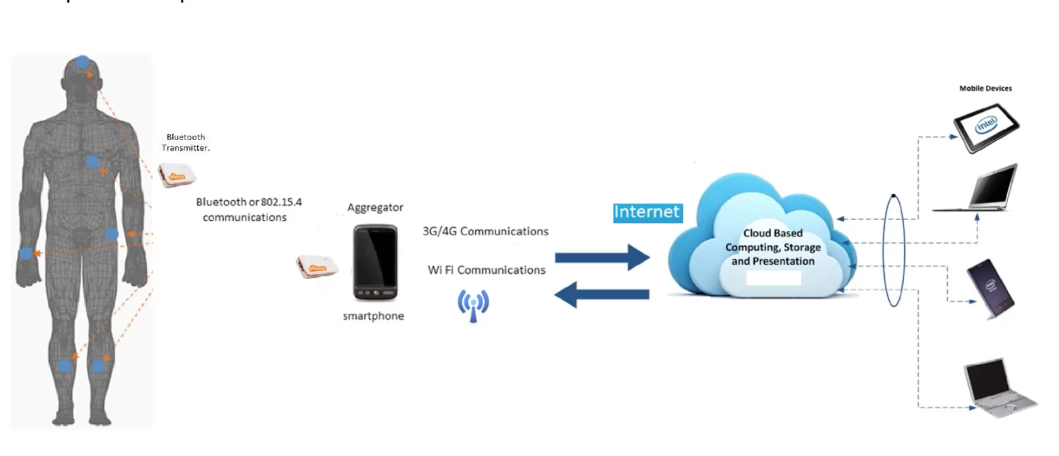
\includegraphics[scale=0.4]{imag/ArquitecturaREF.png}
\caption{Arquitectura de referencia. } %falta asignarREF
\label{3}
\end{figure}
\FloatBarrier

En el presente proyecto se desarrolló para el manejo de datos recibidos desde un dispositivo android, en una aplicación web donde se manejaran el tipo de datos específicos de cada paciente y se encargará de monitorear el volumen respiratorio.

En esta aplicación web el fisioterapeuta puede registrar usuarios, asignar una prescripción por paciente, actualización de prescripciones y visualización de resultados del flujo respiratorio registrado de una fisioterapia respiratoria.




\subsection{Definición de Arquitectura para Sistema Web}

%C1

\subsubsection{Diagrama Contexto del Sistema}

Dados las especificaciones de los servicios de fisioterapia y los requerimientos desarrollados se construye la siguiente arquitectura del sistema general siguiendo el modelado C4 definido

\begin{figure}[ht]
\centering
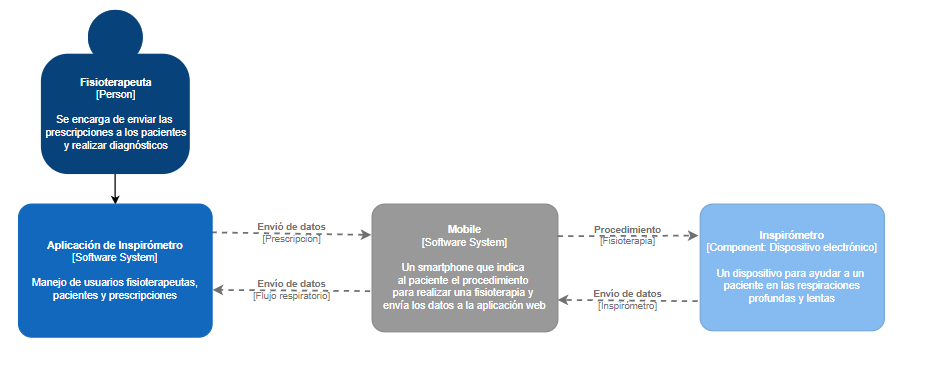
\includegraphics[scale=0.7]{imag/L1C4.PNG}
\caption{Arquitectura de primer nivel del sistema de fisioterapia respiratoria}
\label{5}
\end{figure}
\FloatBarrier

%C2
\subsubsection{Diagrama de Contenedores}
Se identifican funcionalidades especificas del sistema y se separan los servicios:

\begin{figure}[ht]
\centering
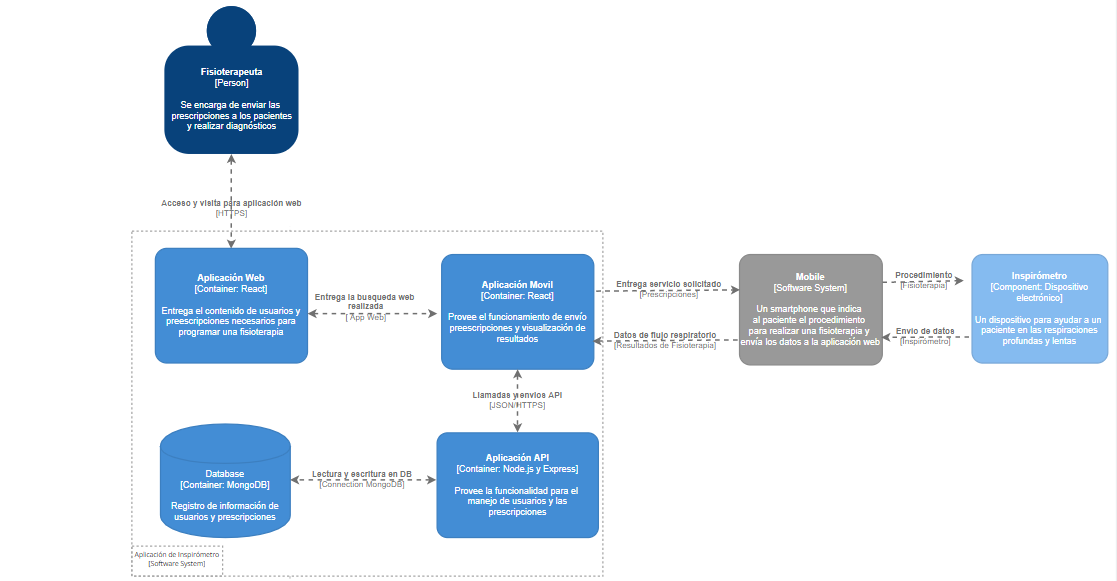
\includegraphics[scale=0.7]{imag/L2C4.PNG}
\caption{Arquitectura de segundo nivel del sistema de fisioterapia respiratoria}
\label{5}
\end{figure}
\FloatBarrier



%C3
\subsubsection{Diagrama de Componentes}


\begin{figure}[ht]
\centering
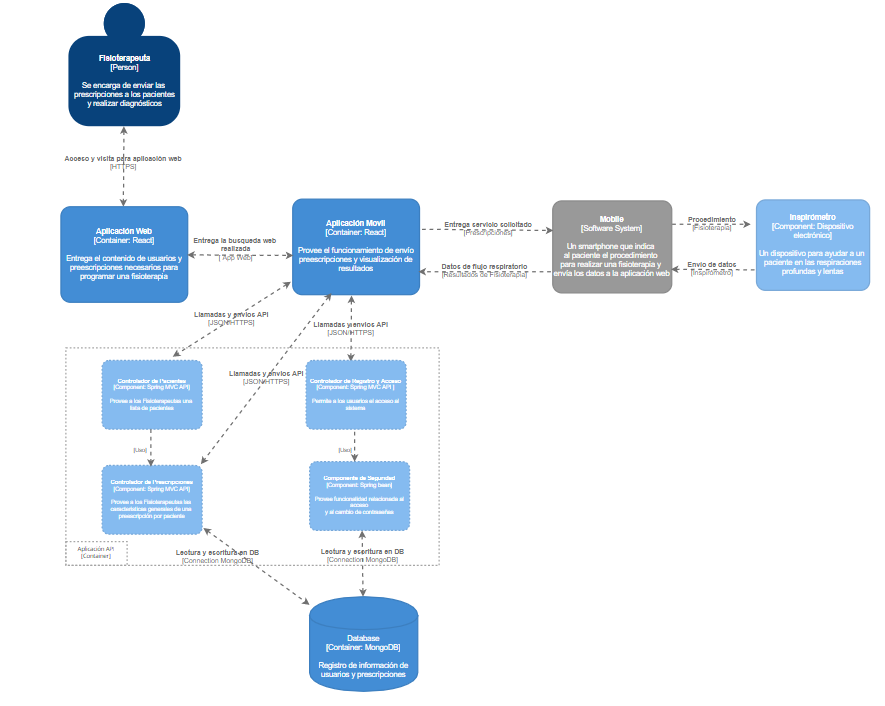
\includegraphics[scale=0.8]{imag/L3C4.PNG}
\caption{Arquitectura de primer tercer del sistema de fisioterapia respiratoria}
\label{5}
\end{figure}
\FloatBarrier



%C4

\subsubsection{Modelo de bases de datos}

%mejorar el
\begin{figure}[ht]
\centering
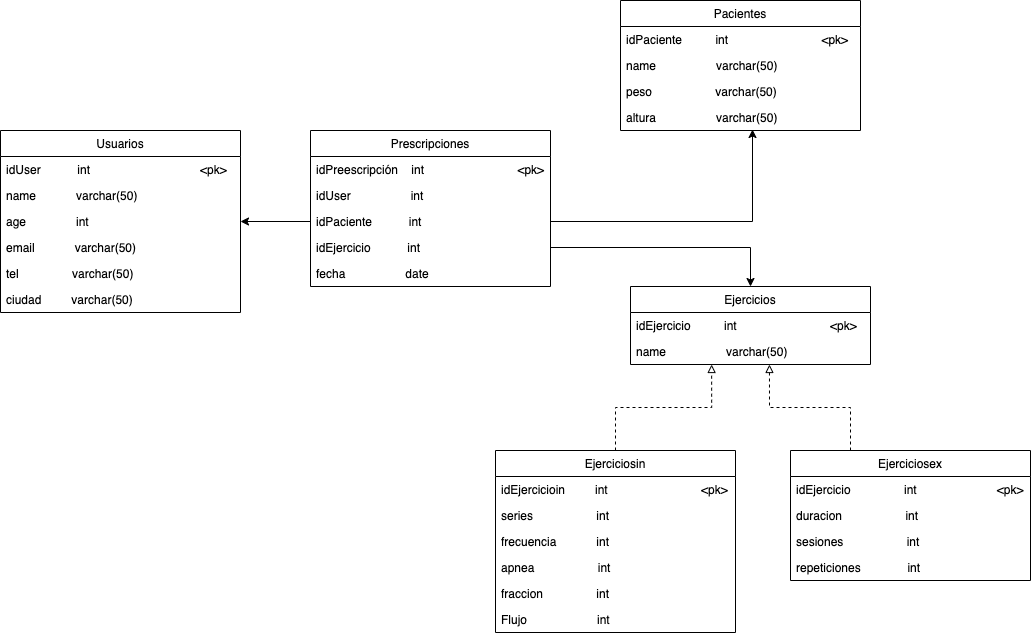
\includegraphics[scale=0.36]{imag/Modelo DB.png}
\caption{Modelo de Base de datos}
\label{6}
\end{figure}
\FloatBarrier


\subsection{Usuarios} Los usuarios en el sistema se definen como usuario tipo paciente o usuario tipo fisioterapeuta
\subsection{Prescripción} La prescripción es establecida por un usuario tipo fisioterapeuta con los datos de un ejercicio de inspiración profunda %validar






\section{Tecnologías de implementación}

Se establece como marco de trabajo de desarrollo, React conocido para la creación de aplicaciones de front end. Este sistema se plantea en dos fases, la primera como inicio de desarrollo del sistema software en entorno de trabajo local y la segunda en un entorno de trabajo online donde se trabajara con las herramientas virtuales presentadas en este capitulo.

%REACT
%C1
\begin{figure}[ht]
\centering
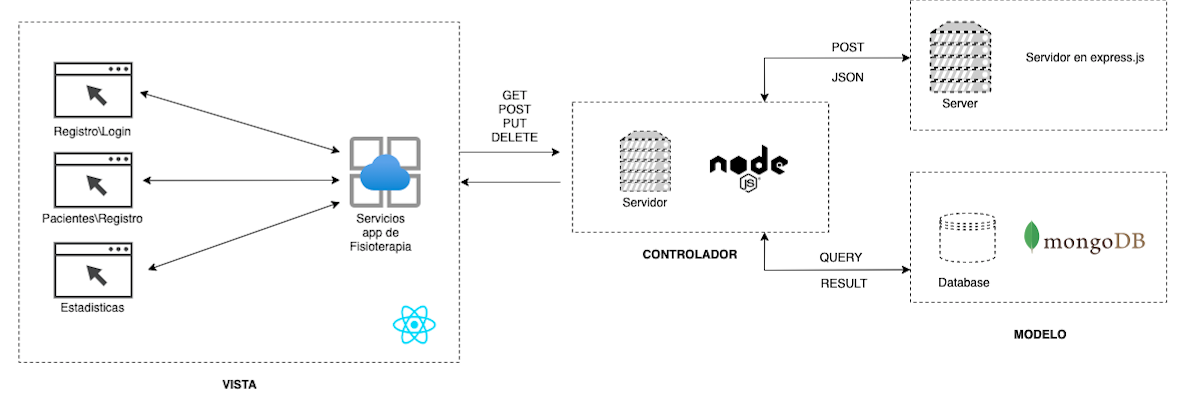
\includegraphics[scale=0.36]{imag/React1.png}
\caption{Arquitectura con tecnologías definidas }
\label{6}
\end{figure}
\FloatBarrier





\subsection{Database MongoDB}

%REACT
%C1
\begin{figure}[ht]
\centering
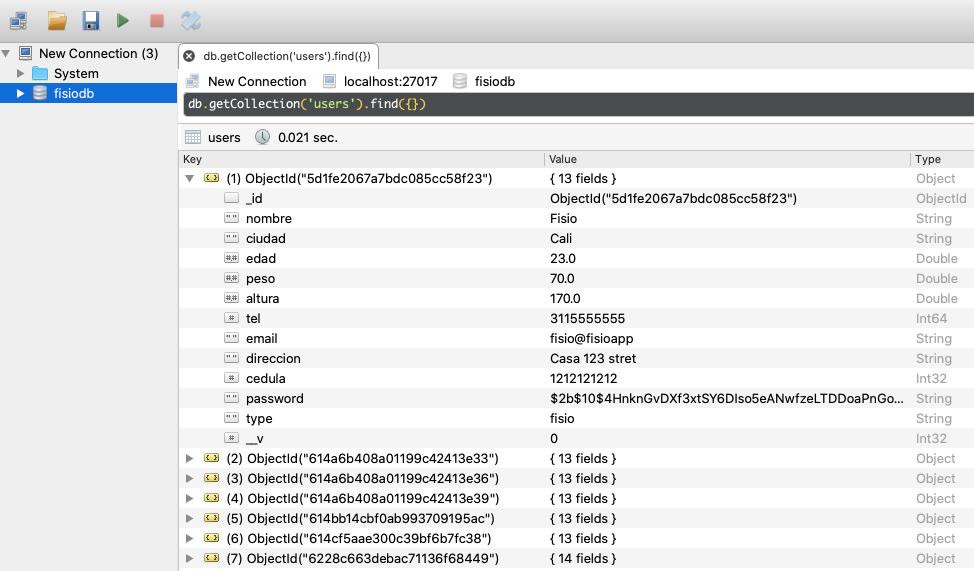
\includegraphics[scale=0.36]{imag/databasemongo.png}
\caption{Base de datos en mongo }
\label{6}
\end{figure}
\FloatBarrier







\section{Proyecto API}


\subsection{Comunicación local entre aplicación Web y API}

\begin{enumerate}
    \item \textbf{Servicio de autenticación:} El el usuario valido es el usuario tipo fisioterapeuta y tipo paciente con el nombre del servicio authenticateUser, con la petición en el ejemplo de a continuación se obtiene el token, el cual sera necesario para acceder a los otros servicios que requieren. autorización.
            \begin{figure}[ht]
            \centering
            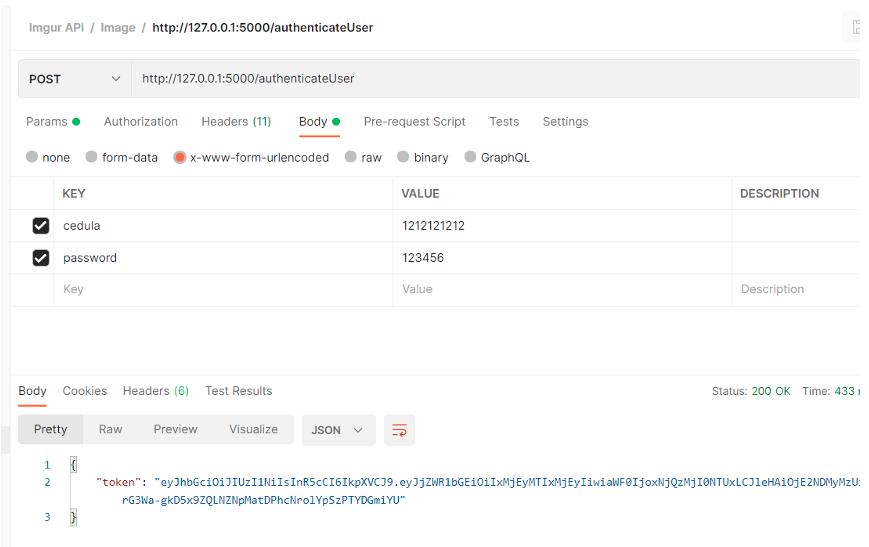
\includegraphics[scale=0.4]{imag/POSTAUS.png}
            \caption{Petición http post en postman para usuario fisioterapeuta}
            \label{6}
            \end{figure}
            \FloatBarrier
            
            \begin{figure}[ht]
            \centering
            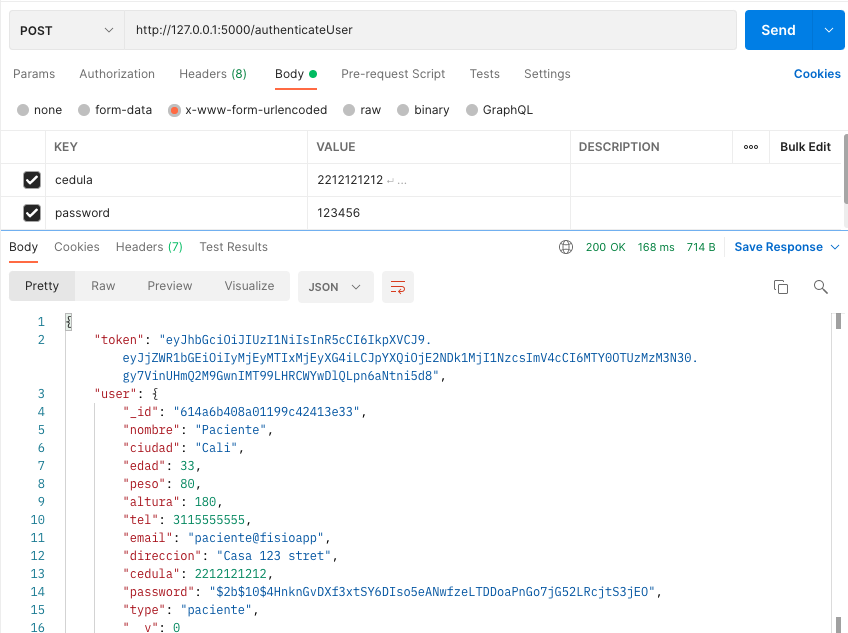
\includegraphics[scale=0.4]{imag/pacienteau.png}
            \caption{Petición http post en postman para usuario paciente}
            \label{6}
            \end{figure}
            \FloatBarrier
            
    \item \textbf{Servicio de consulta a todos los pacientes} Para obtener el id del usuario del cual se requiere consultar su prescripción se llama el servicio allUsers, enviando el token obtenido en el paso anterior.
    
            \begin{figure}[ht]
            \centering
            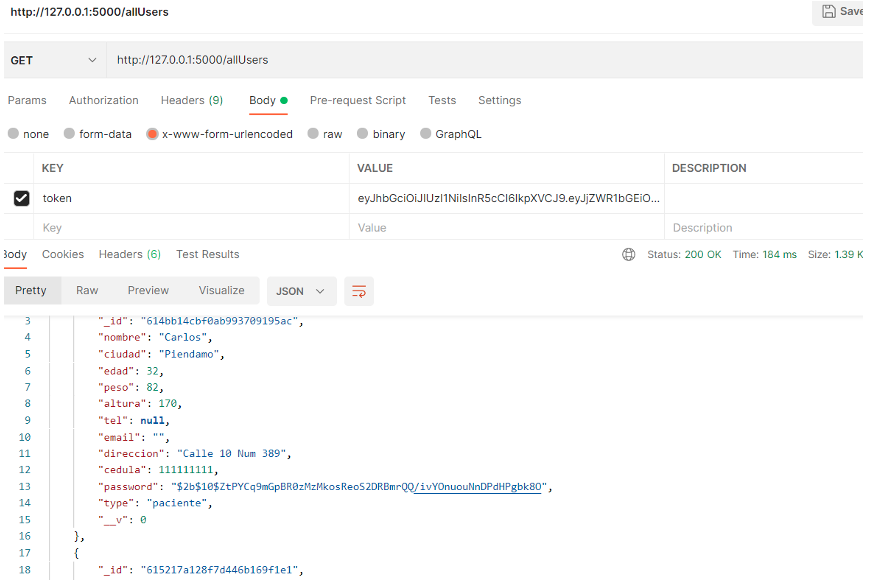
\includegraphics[scale=0.4]{imag/allus.png}
            \caption{Petición get en Postman }
            \label{6}
            \end{figure}
            \FloatBarrier
            
    \item \textbf{Servicio de prescripción}  Para obtener la prescripción de un paciente donde se muestran los ejercicios recomendados se hace el llamado al servicio allEjerciciosByUser enviando los datos como se muestran en el siguiente ejemplo. El resultado muestra los datos de la prescripción para el paciente, el campo que esta marcado como null, no es considerado para ningún efecto. En este caso en particular el token se programó para expirar en 3 horas si no se hace ninguna petición en este lapso.
    
            \begin{figure}[ht]
            \centering
            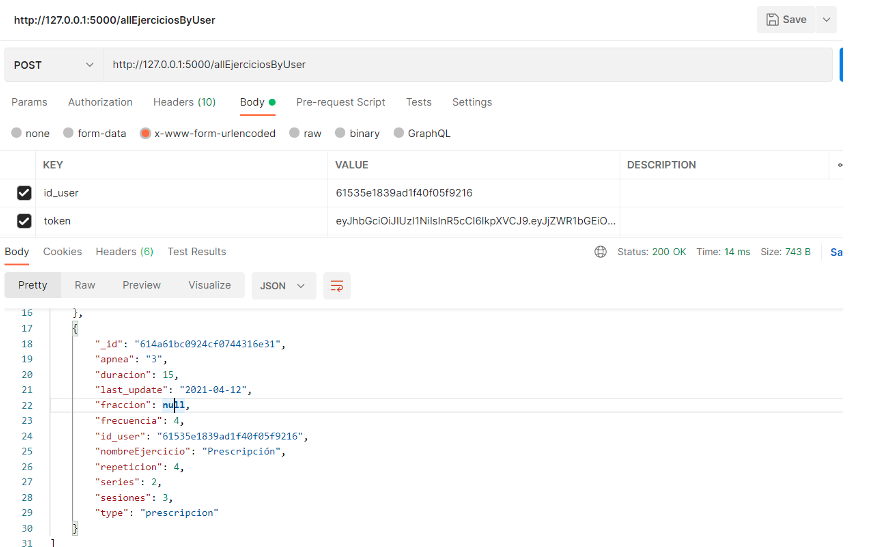
\includegraphics[scale=0.4]{imag/prees.png}
            \caption{Petición post en Postman }
            \label{6}
            \end{figure}
            \FloatBarrier
    



\end{enumerate}


\subsection{Servidor Virtual}

Para dejar el proyecto API en la nube y tener la url publica para el acceso del usuario final, se crea el servidor virtual en AWS lightsail, lo cual es una herramienta que brinda la creación y gestión de instancias para aplicaciones web. En este caso contamos con dos instancias una para la base de datos y otra para la aplicación.

\begin{figure}[ht]
\centering
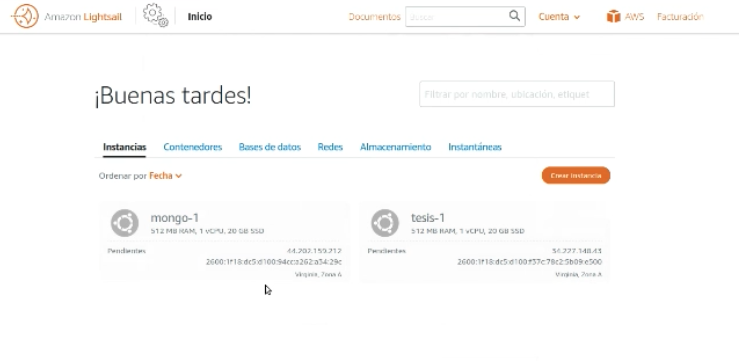
\includegraphics[scale=0.4]{imag/maquinasAWS.png}
\caption{Creación de instancias en AWS }
\label{6}
\end{figure}
\FloatBarrier


Por lo tanto, se puede gestionar como una red virtual privada para que la aplicación web se conecte con la base de datos y se pueda gestionar su acceso mediante la vinculación con una IP estática .

\begin{figure}[ht]
\centering
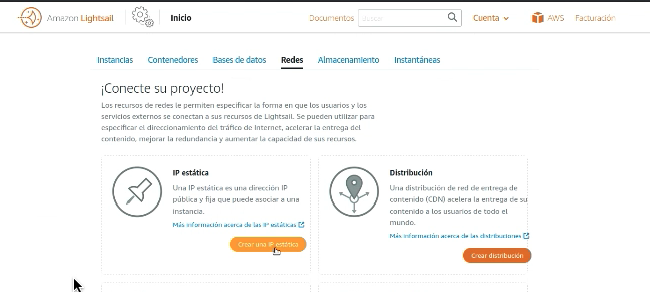
\includegraphics[scale=0.4]{imag/IPestaticaAWS.png}
\caption{Creación de instancias AWS }
\label{6}
\end{figure}
\FloatBarrier

Entonces la url se encuentra funcionando para una carga moderada de trabajo en: %definir cantidad de carga o peticiones

\begin{figure}[ht]
\centering
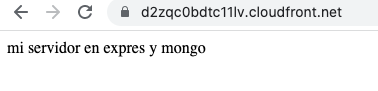
\includegraphics[scale=0.4]{imag/onlineaws.png}
\caption{Proyecto API en AWS}
\label{6}
\end{figure}
\FloatBarrier


\subsection{Comunicación online entre aplicación Web y API}


\subsection{Peticiones web con nodemon}



%prototipos iniciales del sistema






\section{Prototipo Funcional del Sistema Web }

\subsection{Servicios Implementados}




\subsection{Librerias de React}

\subsection{Aplicación Web}

En esta sección se presenta el prototipo funcional del sistema donde se especifica en detalle las funcionalidades

\subsubsection{Registro usuarios}

El fisioterapeuta tiene fijada una lista de pacientes que se presenta por cédula y por nombre, en esta vista de la interfaz, el fisioterapeuta puede ver la prescripción del paciente seleccionado, eliminar o registrar un paciente ver su prescripción.

\begin{figure}[ht]
\centering
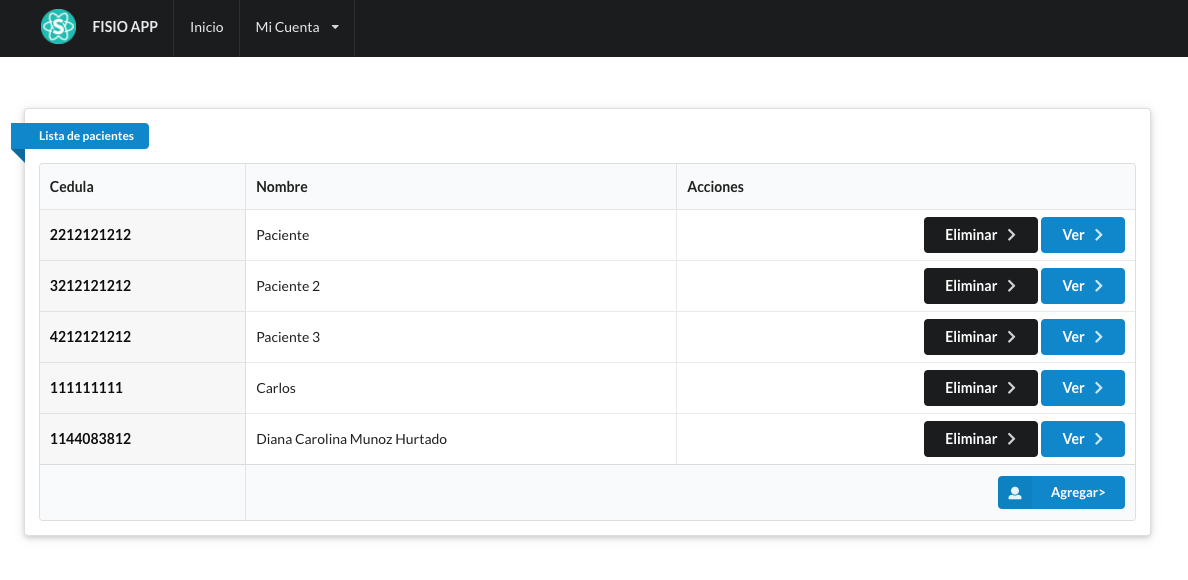
\includegraphics[scale=0.36]{imag/listpacientes.png}
\caption{Lista de pacientes}
\label{6}
\end{figure}
\FloatBarrier

Para registrar un nuevo paciente se requiere los datos que se muestran a continuación:

\begin{figure}[ht]
\centering
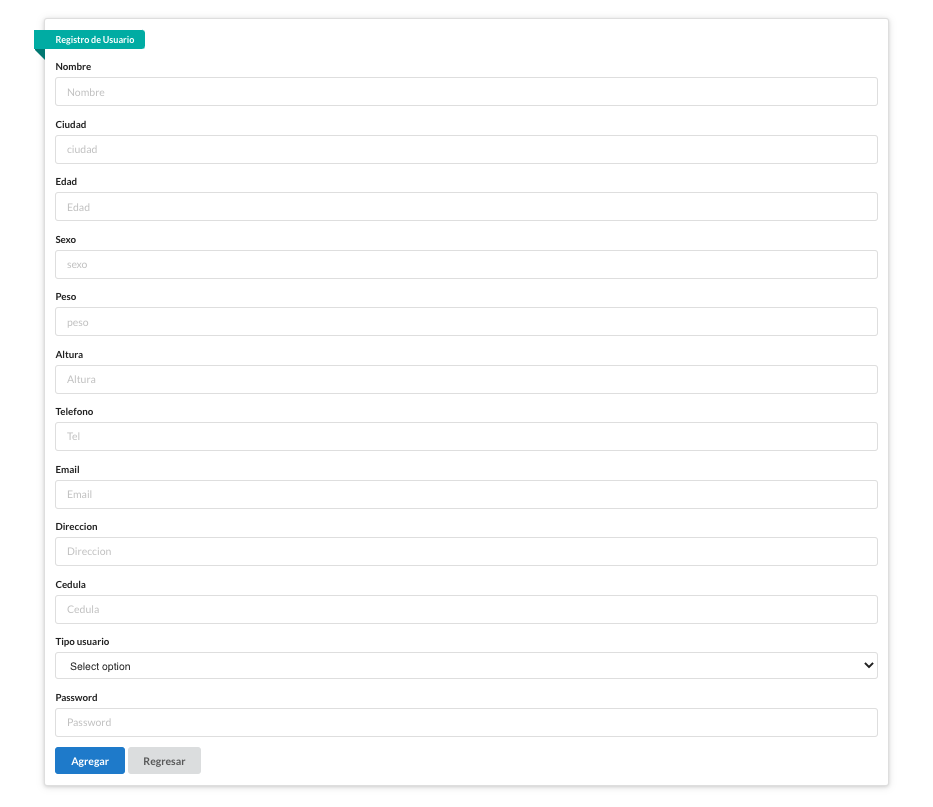
\includegraphics[scale=0.4]{imag/registrousaapp.png}
\caption{Registro de pacientes}
\label{6}
\end{figure}
\FloatBarrier




\subsubsection{Inicio de sesión para usuarios}


\subsubsection{Prescripción a pacientes}


En la prescripción del paciente el fisioterapeuta podrá ver para el paciente seleccionado, la capacidad vital calculada por el sistema dados los datos del paciente, también puede ver los indicadores de fisioterapia que han sido asignados al paciente previamente.

\begin{figure}[ht]
\centering
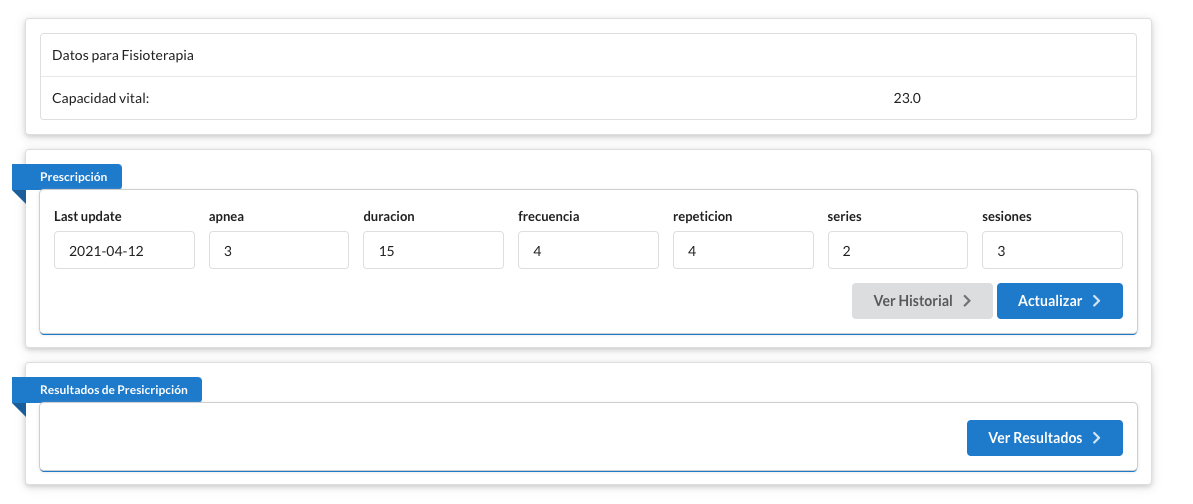
\includegraphics[scale=0.36]{imag/prescriapp.png}
\caption{Prescripción asignada a un paciente}
\label{6}
\end{figure}
\FloatBarrier


\subsubsection{Visualización de resultados}

Se presenta la curva de volumen vs tiempo de una fisioterapia realizada; la gráfica de a continuación muestra los datos de prueba:

\begin{figure}[ht]
\centering
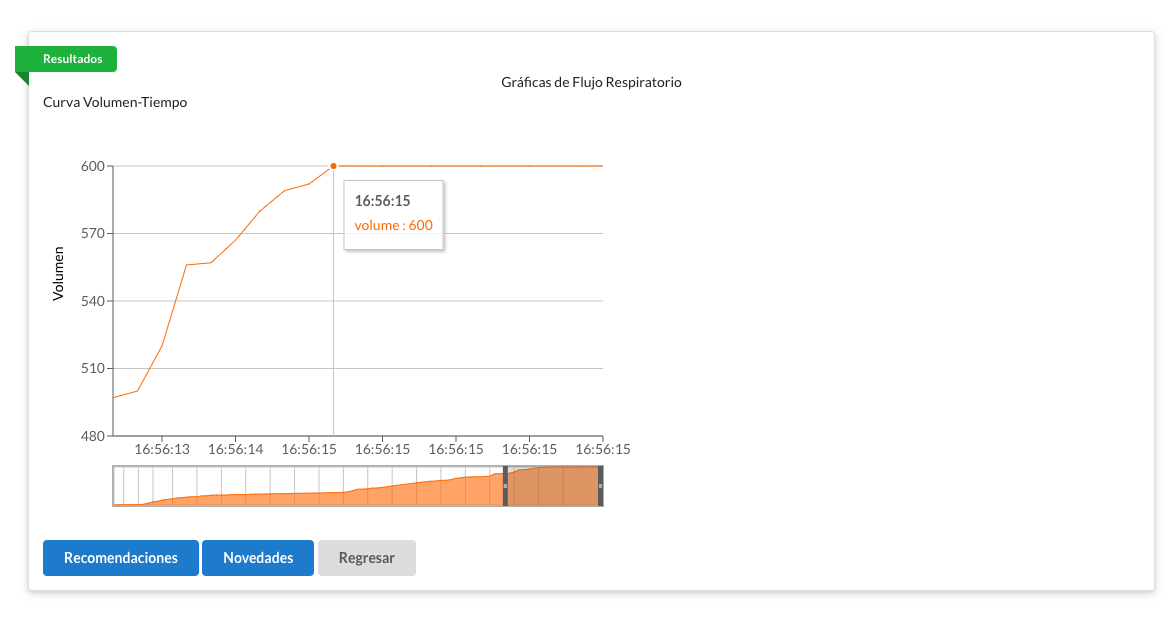
\includegraphics[scale=0.43]{imag/volumetiempoapp.png}
\caption{Visualización de flujo respiratorio}
\label{6}
\end{figure}
\FloatBarrier






\subsubsection{Fase de comunicación y pruebas}

Se envía el ID del usuario  (en la colección de usuarios de mongo DB el campo id)y se reciben los datos de inspiración y espiración para graficar, necesito saber el nombre del nombre de la función y la URL donde esta ubicada


%\subsection{Análisis estadístico de datos}

\subsection{Resultados de fisioterapia}



%-------------------------------------------------------------------------------------
\section{Conclusiones y Recomendaciones}


\section{Trabajos Futuros}




\newpage



%%%%%%%%%%%%%%%%%%%%%%%%%%%%%
% BIBLIOGRAFIA
%%%%%%%%%%%%%%%%%%%%%%%%%%%%%
\bibliography{biblio.bib}
\bibliographystyle{IEEEtran}
\nocite{1}
\nocite{2}
\nocite{3}
\nocite{4}
\nocite{5}

%%%%%%%%%%%%%%%%
% GENERAL INDEX
%%%%%%%%%%%%%%%%
%\printindex



\section{Anexos}
\subsection{Prototipo Inicial del Sistema Web} 


\begin{figure}[ht]
\centering
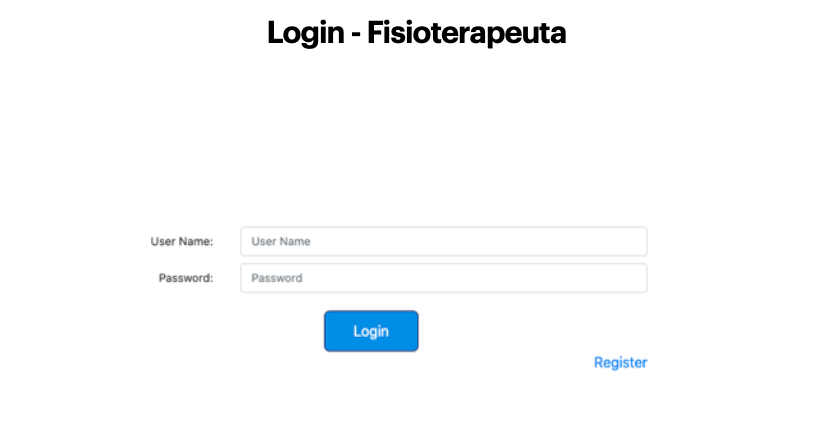
\includegraphics[scale=0.4]{imag/P1.png}
\caption{Login }
\label{6}
\end{figure}
\FloatBarrier

\begin{figure}[ht]
\centering
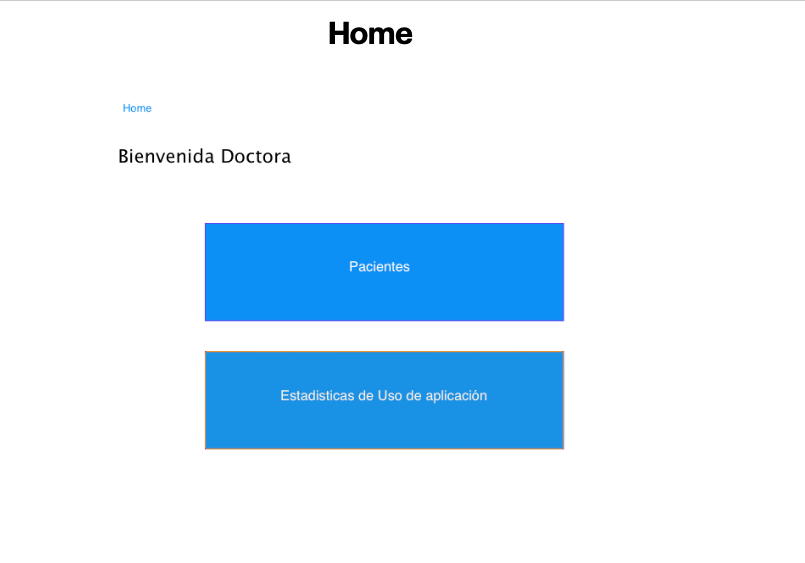
\includegraphics[scale=0.4]{imag/P3.png}
\caption{Menú principal }
\label{6}
\end{figure}
\FloatBarrier


\begin{figure}[ht]
\centering
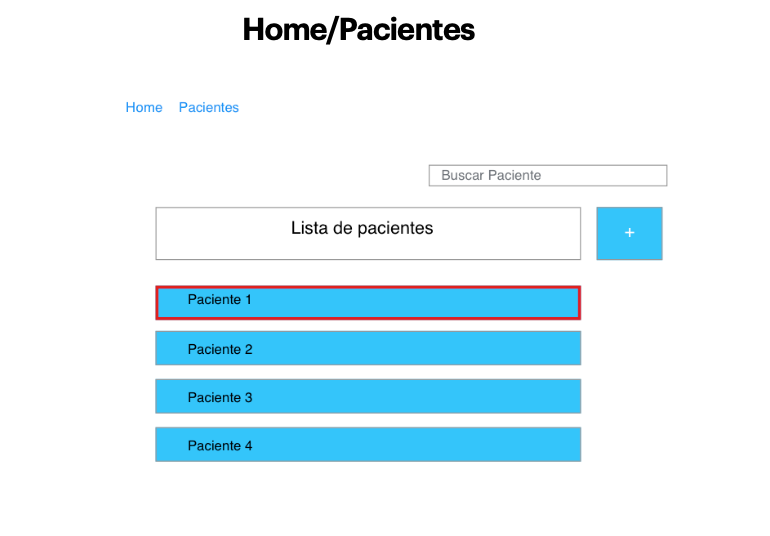
\includegraphics[scale=0.4]{imag/P4.png}
\caption{Lista de pacientes }
\label{6}
\end{figure}
\FloatBarrier


\begin{figure}[ht]
\centering
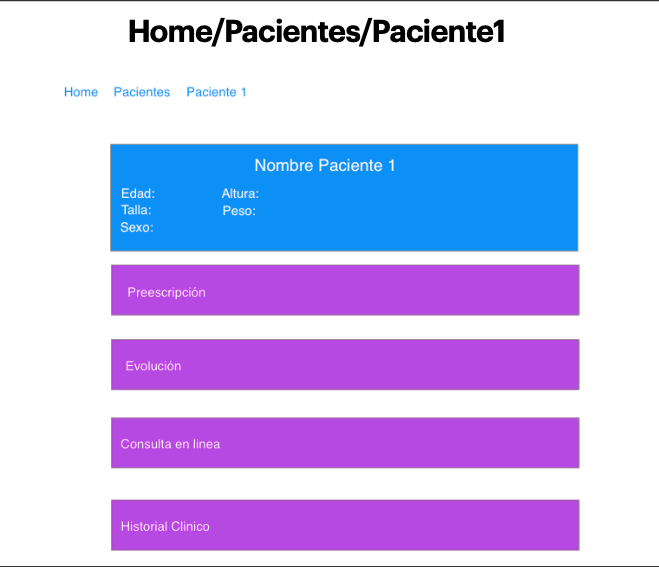
\includegraphics[scale=0.4]{imag/P5.png}
\caption{Modelo de paciente 1 }
\label{6}
\end{figure}
\FloatBarrier


\begin{figure}[ht]
\centering
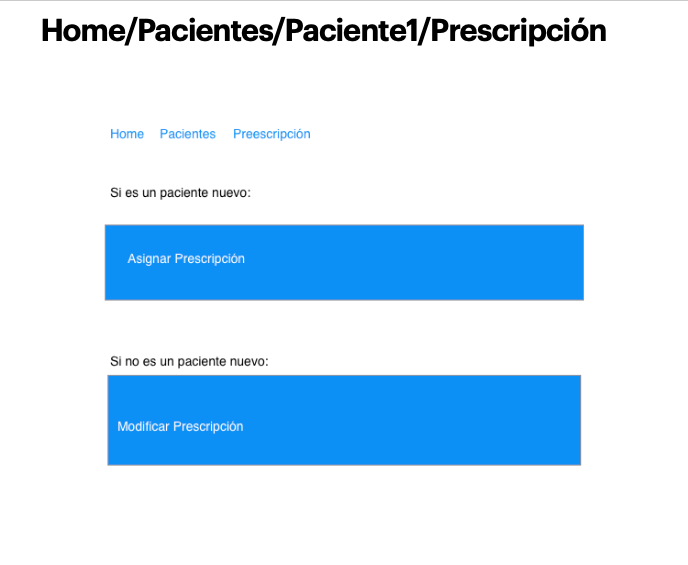
\includegraphics[scale=0.4]{imag/P6.png}
\caption{Modelo de prescripción  }
\label{6}
\end{figure}
\FloatBarrier


\begin{figure}[ht]
\centering
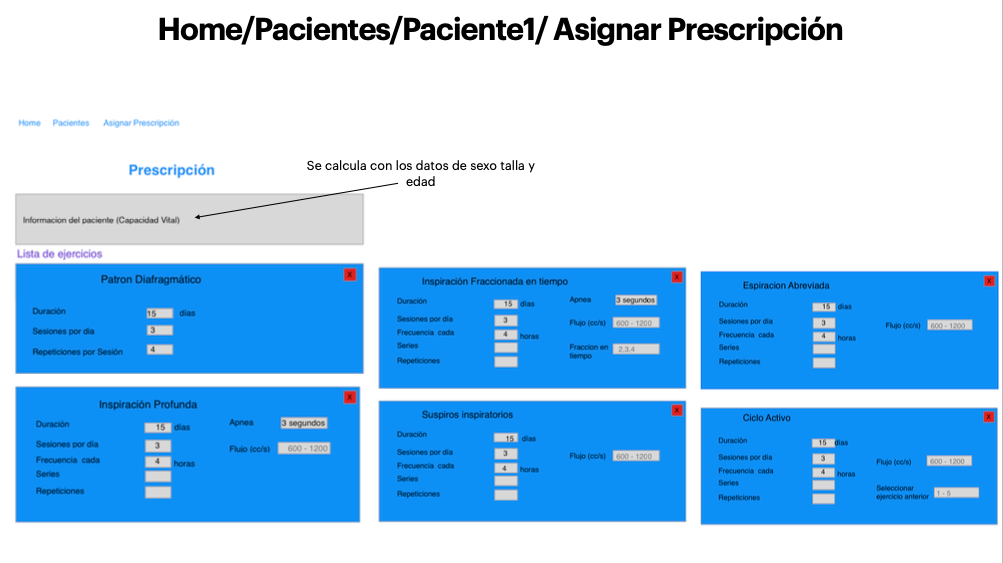
\includegraphics[scale=0.4]{imag/P7.png}
\caption{Modelo de asignar prescripción }
\label{6}
\end{figure}
\FloatBarrier


\begin{figure}[ht]
\centering
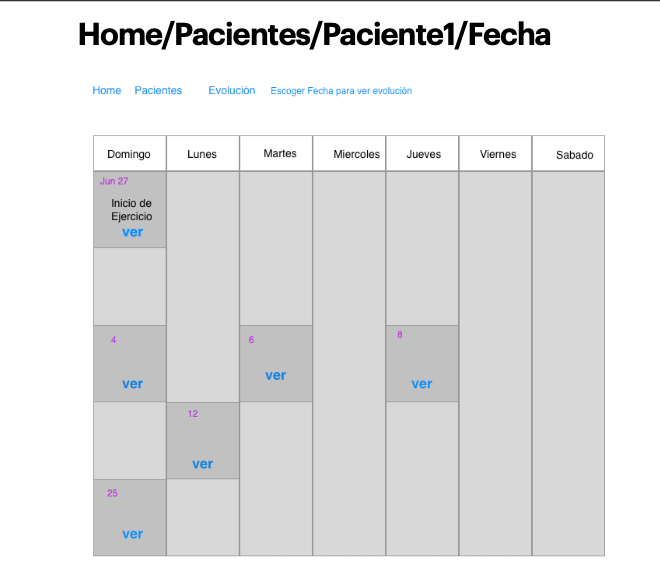
\includegraphics[scale=0.35]{imag/P8.png}
\caption{Modelo de registro de fecha }
\label{6}
\end{figure}
\FloatBarrier


\begin{figure}[ht]
\centering
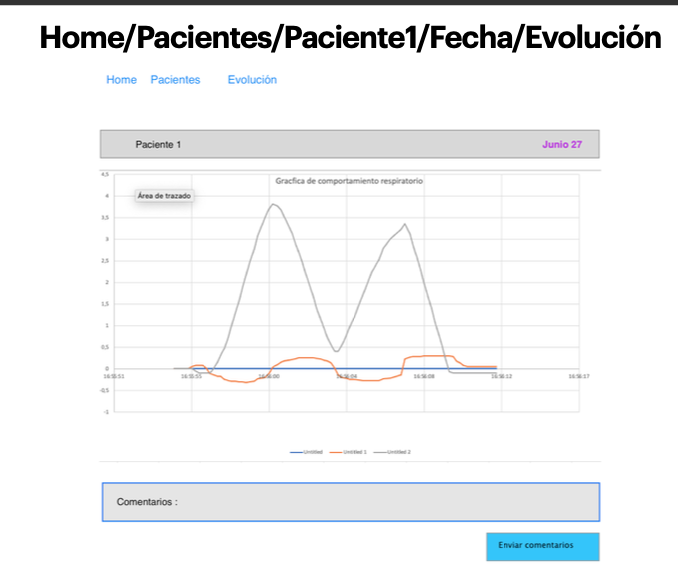
\includegraphics[scale=0.4]{imag/P9.png}
\caption{Modelo de Evolución del Paciente }
\label{6}
\end{figure}
\FloatBarrier


\begin{figure}[ht]
\centering
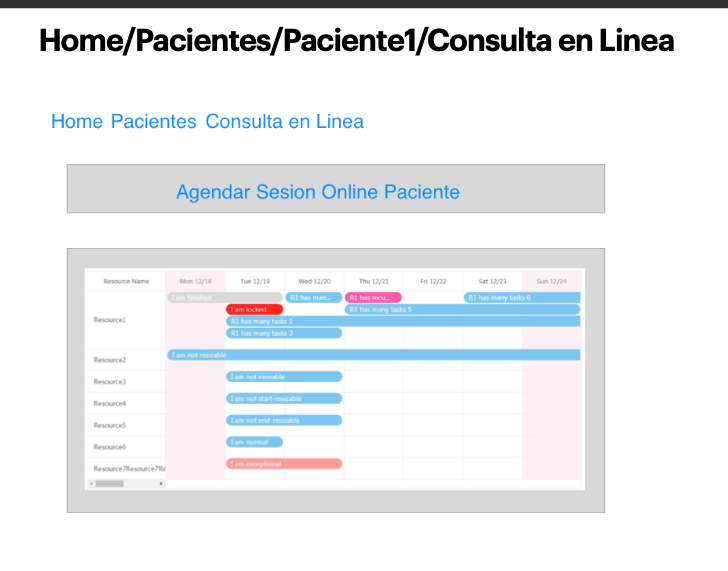
\includegraphics[scale=0.4]{imag/P10.png}
\caption{ Modelo de realizar consulta en línea}
\label{6}
\end{figure}
\FloatBarrier



\begin{figure}[ht]
\centering
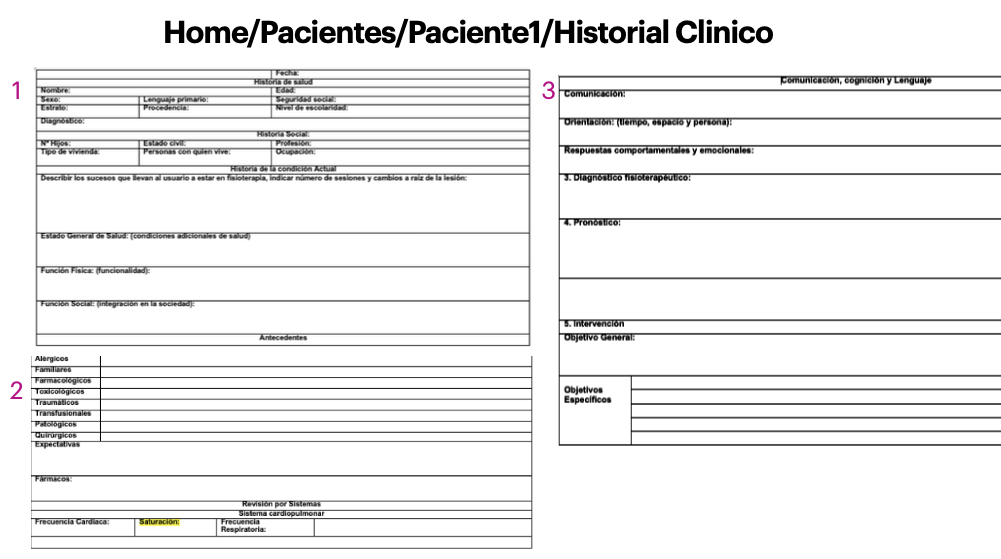
\includegraphics[scale=0.36]{imag/P11.png}
\caption{Modelo de Historial Clínico }
\label{6}
\end{figure}
\FloatBarrier


\begin{figure}[ht]
\centering
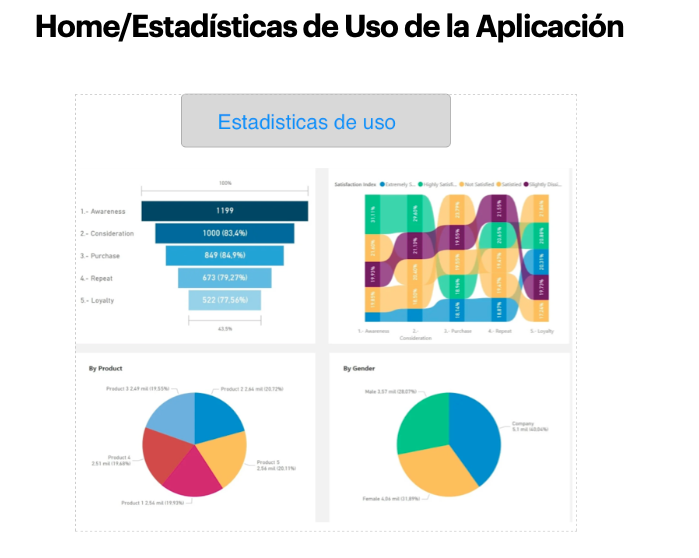
\includegraphics[scale=0.36]{imag/P12.png}
\caption{Modelo de Estadísticas de Uso de la aplicación }
\label{6}
\end{figure}
\FloatBarrier







\end{document}


